%% Bachelor Thesis Template of Wuhan Uniersity
%%
%% Created by Fing

\documentclass[]{WHUBachelor}
\usepackage{multirow}
\usepackage{url}
\usepackage{mathrsfs}
%\usepackage{algorithm}  
%\usepackage{algorithmicx}  
%\usepackage{algpseudocode}  
%\usepackage{amsmath}  

%\floatname{algorithm}{算法}  
\renewcommand{\algorithmicrequire}{\textbf{输入:}}  
\renewcommand{\algorithmicensure}{\textbf{输出:}}  
 
\begin{document}
%%----------- 封面部分 ----------- %%
  
  \stunum{2016301500030}
  \ctitle{一种图像-语义互译系统}
  \cschool{弘毅学堂}
  \cmajor{计算机科学与技术}
  \cauthor{雷伯涵}
  \cadvisor{庄越挺\quad 教\quad  授}
  \caadvisor{黄\quad 浩\quad 副教授}
  %\cadvisor{黄浩\quad 副教授}
  \cdate{二〇二〇年五月}

  %\stunumE{Lei, Bohan}
  \ctitleE{An Image-Languange Traslation System}
  \cschoolE{Hongyi Honored School}
  \cmajorE{Computer Schience and Technology}
  \cauthorE{Lei, Bohan}
  \cadvisorE{Prof.\hspace{2.5em}Zhuang, Yueting}
  \caadvisorE{Asso Prof. Huang, Hao}
  \cdateE{MAY 2020}

  \maketitlepage            % 封面
  \maketitlepageE           % 封面
  \makestatement            % 申明

%%----------- 前言部分 ----------- %%
  % 中英文摘要

\begin{cnabstract}{推荐算法;深度学习;个性化推荐;DeepFM}
  随着互联网的日渐普及,数据积累越来越丰富,已出现过载的现象。如何合
理有效地挖掘数据的潜在价值,以辅助推动经济增长,是当前的一个热门话题。

  相比之需要用户抱有明确目的性去筛选信息的搜索引擎,推荐技术可以借助
用户人口统计学属性和其交互行为等数据进行相关分析,进而实现自动地为用户
推荐他们需求的信息的效果。鉴于此,推荐技术在近些年来一直是研究热点,其
也随着时代日新月异。

本文基于推荐算法研究的考量,结合博物馆观众服务质量有待提高的需求,
深入探究了基于因子分解机的神经网络模型框架。并基于此框架和深度神经网络 构建了 DeepFM-D 模型,实现了一种面向博物馆观众服务的个性化推荐。

本文对课题实验结果作了相关分析,从预测评分准确性和推荐列表输出准确 
性两个角度出发,利用 FM、DNN 等不同算法模型在此评估标准上与 DeepFM-D 模型进行了推荐对比实验。实验结果表明,DeepFM-D 模型评估指标具有较明显 的优势,其效果的有效性得到验证。
\end{cnabstract}

\begin{enabstract}{Recommendation Algorithm; Deep Learning; Personalized Recommendation; DeepFM}
With the increasing popularity of the Internet, the accumulation of data is becoming more and more abundant, and there has been an overload phenomenon. How to mine the potential value of data reasonably and effectively to help promote economic growth is currently a hot topic.

In contrast to search engines that require users to have a clear purpose to filter information, recommendation techniques can use data such as user demographic attributes and their interactive behaviors to perform relevant analysis, thereby achieving the effect of automatically recommending the information they need for users. In view of this, recommendation technology has been a research hotspot in recent years, and it also develops rapidly with the times.

In this paper, based on the consideration of the research of recommendation algorithms, combined with the needs of museum audience service quality to be improved, the neural network model framework based on factorization machine is deeply explored. Based on this framework and deep neural network, the DeepFM-D model is constructed to realize a personalized recommendation for museum audience services.

This paper makes a relevant analysis of the experimental results of this subject. From two perspectives of the accuracy of prediction scores and the accuracy of the output of the recommendation list, different algorithm models such as FM and DNN are used to compare and recommend the DeepFM-D model on this evaluation standard. The experimental results show that the evaluation index of DeepFM-D model has obvious advantages, and the effectiveness of its effect is verified.

\end{enabstract}
  % 摘要
  \contents                 % 目录
 
%%----------- 主体部分 ----------- %%
  %Chapter 1

  % chapter 2

\chapter{相关技术理论}

\section{引言}
设计中的两个翻译技术均由深度学习的模型训练得出,本章具体介绍图片翻译文本技术和文本翻译图片技术的前置理论。

图片翻译文本技术的主体使用了编码-解码架构的长短期记忆模型。长短期记忆模型是一种特殊的循环神经网络,接下来首先将详细介绍神经网络、循环神经网络、长短期记忆的原理和模型结构,并阐述长短期记忆适用于文本生成的援引。文本翻译图片技术的主体使用了GAN网络模型。由于GAN网络模型在图片生成的领域内已经有了几个大的突破,我将在介绍GAN模型的结构和原理后,介绍相关的GAN模型的分支优化算法在图片生成领域的表现。

\section{图片翻译文本相关工作}
本次设计中图片字幕技术部分主要使用的技术基于长短期记忆循环神经网络。这一小节将阐述循环神经网络和长短期记忆的相关技术。
\subsection{神经网络}
神经网络(Neural Networks)是近年比较流行的概念。在2006年Hiinton\upcite{hinton2006reducing}提出深度学习概念后,成为了优化算法表现性能的一大利器。

神经网络的基本结构就是由神经元构成的网络,每个神经元结构如图~\ref{fig:nnc}所示,输入输出关系如式\eqref{eq:nn}表述结果。
\begin{equation}
    \label{eq:nn}
    f( \sum\limits_{i=1}^{m} w_i x_i + b ) 
\end{equation}
其中,$w$是神经网络上的边权(weight),$x$代表着输入数据,$b$则是神经网络中神经元的偏差值(bias)。

对于第$j$层的每一个神经元,它会对上一层的每一个神经元输入的$x_i$赋予权重$w_i$,计算出输出结果,即如式\eqref{eq:nnj}所示,其中n是每一层的神经元个数,由输入神经元个数决定。
\begin{equation}
    \label{eq:nnj}
    x_k^j = \sum\limits_{i=1}^{n} w_ik x_ik, k\in \left[1,n\right]
\end{equation}

\begin{figure}[b]
    \centering
    \begin{minipage}[t]{0.4\linewidth}
        \centering
        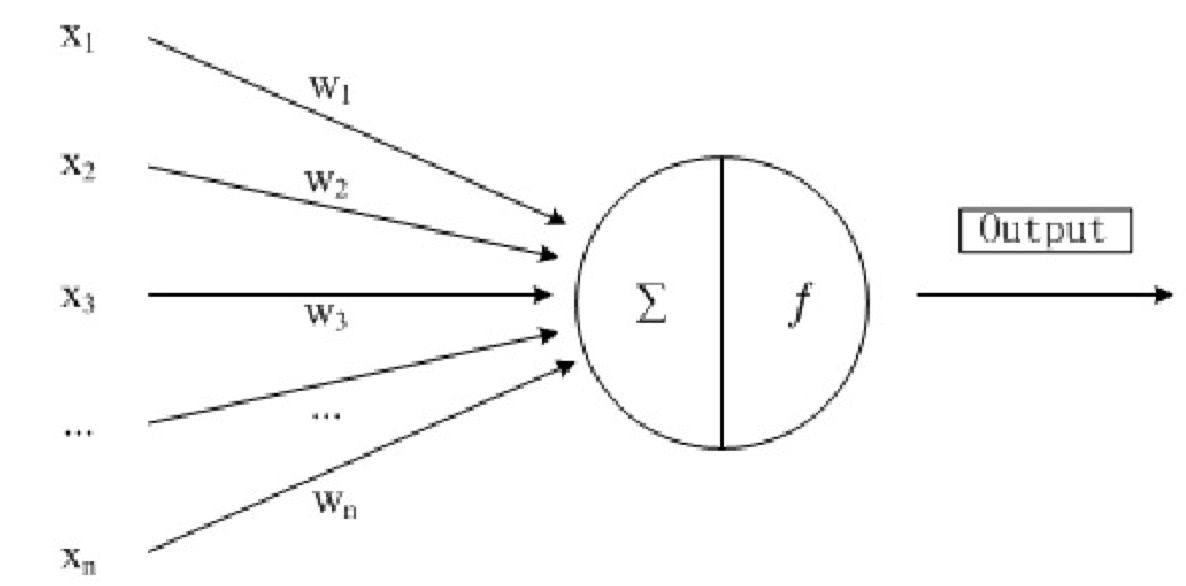
\includegraphics[width=0.9\textwidth]
        {figures/nnc.png}\\
        \caption{神经网络神经元}
        \label{fig:nnc}
    \end{minipage}
    \begin{minipage}[t]{0.5\linewidth}
        \centering
        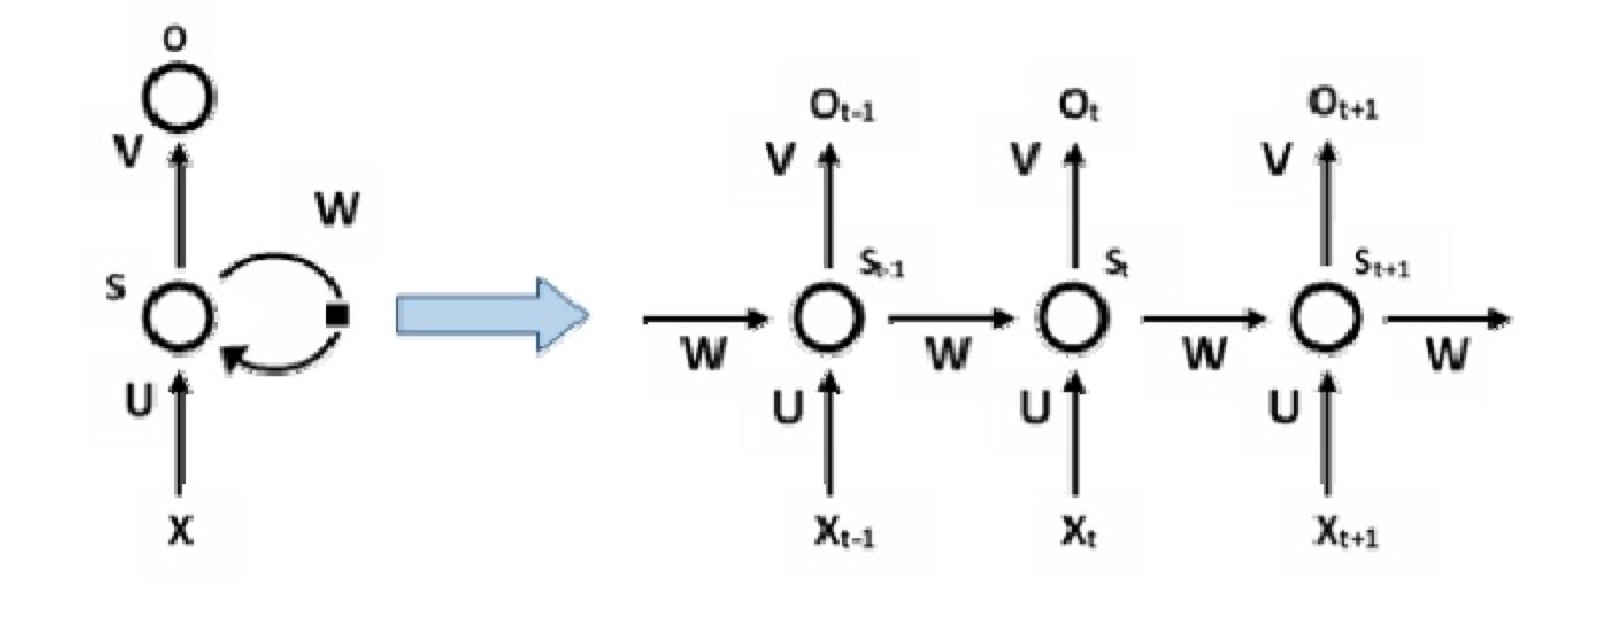
\includegraphics[width=0.9\textwidth]
        {figures/rnnc.png}\\
        \caption{循环神经网络神经元}
        \label{fig:rnnc}
    \end{minipage}
\end{figure}

\subsection{循环神经网络}
循环神经网络(Recurrent Neural Networks, RNN)是一种特殊的神经网络。为了加强上文信息对当前节点的影响,循环神经网络对神经元的输入数据增加了上一时序同一神经元的输出数据。它被广泛地运用在图像处理和自然语言处理上。与一般的神经网络相同,它也有前馈层和反馈层,但是它在一般的神经网络基础上增加了基于时序的循环机制。在一般的神经网络中,神经元之间相互独立,但是现实中的信息往往互相关联。所以,循环神经网络的特点像人一样有记忆的能力它的输出不仅依靠当前输入,也依靠历史的输出。在一定程度上,它更能反应真实的情况。

RNN神经元的结构与BP神经网络神经元有些许不同。如图~\ref{fig:rnnc}所示,任一隐藏层中神经元的输出信息依靠当前时刻的输入信息和前序时序的输出信息决定,同时当前时序的输出信息也会作为下一个神经元的输入。这样的神经网络构建了神经元之间的联系,让数据有了更为有效的依赖关系,优化了信息利用的效率。
每一个神经元的计算方式可以表述为式\eqref{eq:rnn}。其中$x_t$代表$t$时刻神经元的输入,$s_t$代表$t$时刻神经元的状态,$o_t$代表$t$时刻神经元的输出。
\begin{equation}
  \begin{split}
    s_t = f(u· x_t + w · s_{t-1}), \\
    o_t = g(s_t·v).\hspace{1.8em} \widetilde{C}_t
  \end{split}
  \label{eq:rnn}
\end{equation}
式中的函数$f$与$g$分别求神经元状态与从状态计算输出值的函数。

%暂时不确定这里放什么图、放不放图
\iffalse %注释开始
\begin{figure}[!htb]
  \centering
  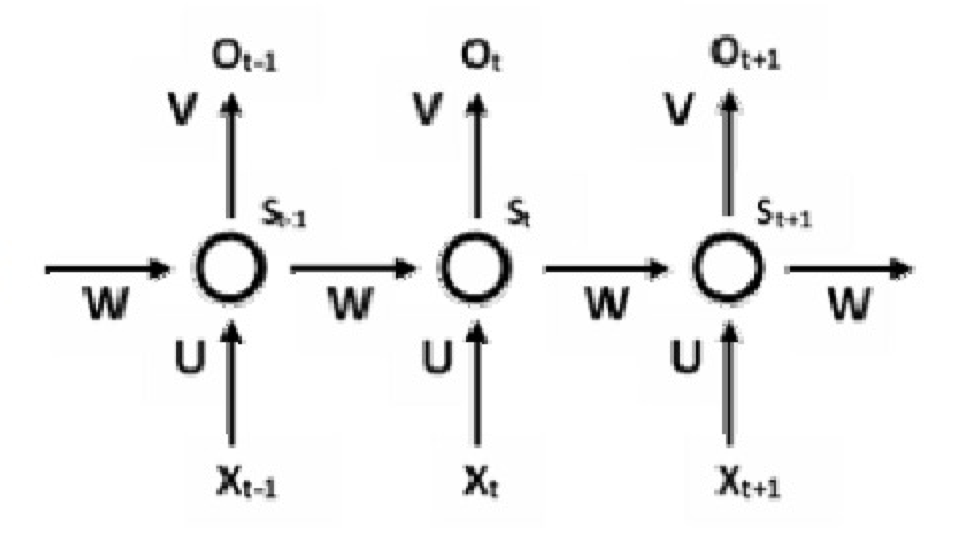
\includegraphics[width=0.6\textwidth]{figures/rnn_net.png}
  \caption{循环神经网络结构}
  \label{fig:rnn}
\end{figure}
\fi %注释结束

\subsection{长短期记忆网络}
从主体上看,LSTM与RNN类似,都是循环神经网络这样的链式结构。而在神经元上看,LSTM细胞节点要比普通的RNN节点要复杂一些。LSTM改进后的神经元由四个不同的神经网络层进行信息的交互,如图~\ref{fig:lstmc}所示。

\begin{figure}[!htb]
  \centering
  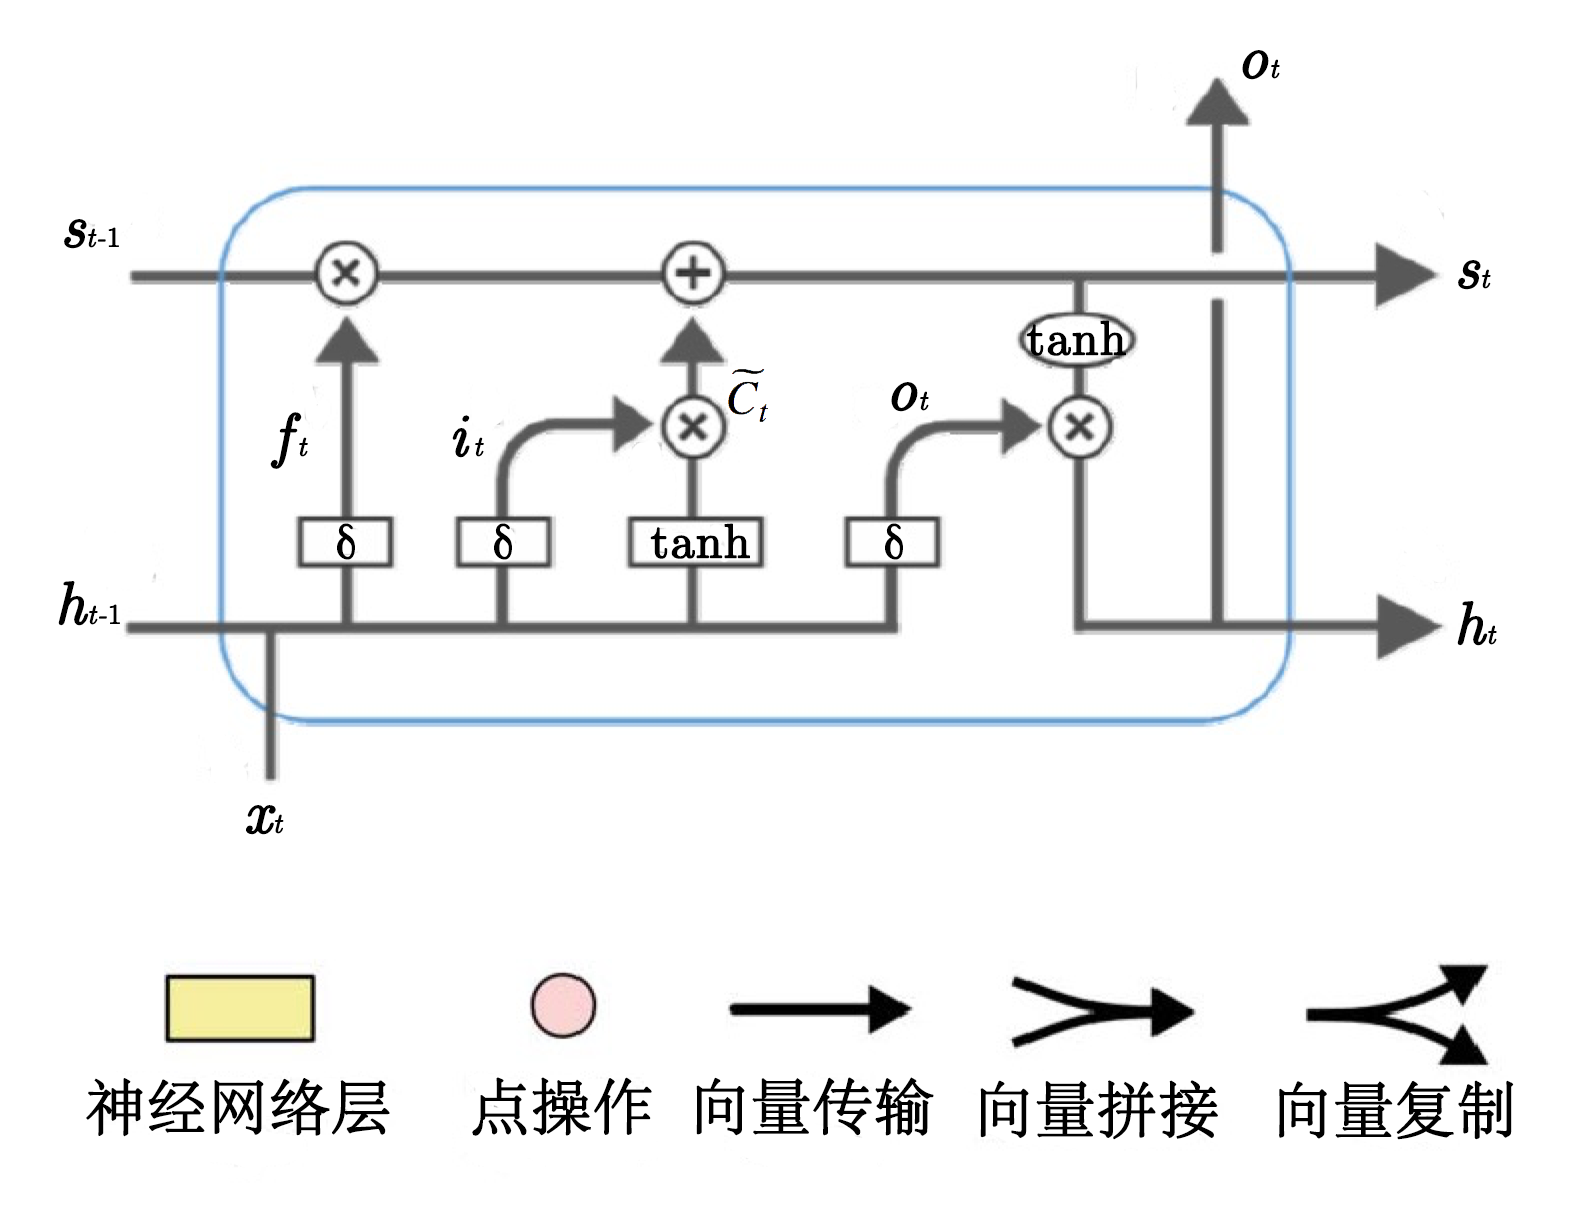
\includegraphics[width=0.6\textwidth]{figures/lstmc.png}
  \caption{LSTM神经元细胞结构图}
  \label{fig:lstmc}
\end{figure}
\hspace{-2em}其中圆形代表基本操作,矩形代表学习得到的状态,箭头代表数据的传输,而箭头的分裂与合并则代表向量的拆分与连接;$s$代表状态,$x$代表输入,$h$代表输出。

在图~\ref{fig:lstmc}中的上方长线段代表了神经网络的状态$s$,它在每个时刻的操作仅在两个地方与输入数据有交互,这就保证了$s$的变化不大,神经元状态比较稳定。LSTM神经元的数据更新由“门”来进行,三个门分别是输入门、遗忘门和输出门,LSTM神经元由此实现数据的更新和储存。

门上的行为由一个点乘Pointwise操作和一个激活函数\textit{Sigmoid}所组成。特别说明,激活函数\textit{Sigmoid}的取值为0至1,分别代表着允许部分信息通过——其中0代表不允许任何信息通过,1代表着允许所有信息通过。

具体的门信息传递机制由以下几个部分完成:
\begin{enumerate}[fullwidth,itemindent=2em,label=\arabic*.]
  %\setlength{\parindent}{4em}
  \item 遗忘门:决定历史信息的保留与遗忘。通过$Sigmoid$函数来决定状态$S$的遗忘程度。
  \begin{equation}
    f_t=\sigma(W_f[h_{t-1}, x_t]+b_f)
    \label{forget}
  \end{equation}
  \item 输入门:决定存储到细胞状态内的新信息。先用$Sigmoid$函数决定记忆的更新程度,然后决定更新的内容,最后将更新的内容加在遗忘内容之上,形成当前时刻的状态。
  \begin{equation}
    \begin{split}
      i_t=\sigma(W_i[h_{t-1}, x_t]+b_i)\hspace{0.2em}\\
      \widetilde{C_t}=\tanh(W_c[h_{t-1}, x_t]+b_c)\hspace{-0.7em}\\
      S_t = f_t·S_{t-1} + i_t · \widetilde{C_t}\hspace{1.1em}
    \end{split}
    \label{input}
  \end{equation}
  \item 输出门:决定输出的值。首先用\textit{Sigmoid}函数决定从状态中输出的部分,然后用$\tanh$对细胞状态进行处理,并与\textit{Sigmoid}函数值相乘,实现输出想输出的部分。
  \begin{equation}
    \begin{split}
      o_t = \sigma(W_o[h_{t-1}, x_t] + b_o)\\
      h_t = o_t*\tanh(S_t)\hspace{1.2em}
    \end{split}
    \label{output}
  \end{equation}
\end{enumerate}
式中,\textit{Sigmoid}函数由模型具体决定,而形如$[\textbf{a}, \textbf{b}]$的操作,代表对两个向量进行拼接(concatenation)。

通过这三个门对神经元的共同作用,LSTM可以完成神经元的基本状态变换,从而完成较好的训练效果。

\section{文本翻译图片相关工作}
文本翻译图片技术中比较原始的模型是CGAN模型\upcite{mirza2014conditional},另一个转折点是Zhang\upcite{zhang2017stackgan}提出的StackGAN模型。本部分将详细阐述GAN的基本原理和在图片生成领域应用的发展历程。

\subsection{GAN模型基本原理}
GANs的基本结构即由一个生成模型$G$和一个判别模型$D$组成。生成模型$G$的目的是尽可能最小化生成与真实训练样本和生成样本的区别,而判别模型$D$的目的则是尽可能最大化地找出真实样本和生成样本之间的区别。

通过多轮迭代生成模型$G$和判别模型$D$的对抗,可以使两个模型都达到上述的目标效果。当训练判别模型$D$的时候,希望输入真实样本$x$可以使判别器对其的判断$D(x)$尽量趋于1,而生成样本$G(x)$通过判别器$D$的时候可以使得$D(G(x))$尽量趋于0。在训练生成模型$G$的时候,输入噪声$z$,希望生成的生成样本通过判别器$D$的时候尽量使得$D(G(z))$趋于0。

可以用简单的数学变换得到公式\eqref{eq:1.1},来描述训练过程。
\begin{equation}
    \label{eq:1.1}
    \min_{G}\max_{D} V_{G,D} = \mathbb{E}_{x \sim P_{data}(x)}[\lg D(x)] + \mathbb{E}_{z \sim P_{G}(z)}[\lg (1-D(G(z)))]
\end{equation}
其中$P_{data}(x)$为真实图片集的分布。

当多轮博弈过后,极大极小问题达到最优解,即纳什均衡,当且仅当$P_z = P_{data}$时\upcite{goodfellow2014generative}。这时$\mathbb{E} D(G(z))$趋于$\frac{1}{2}$,即相当于只能随机猜测0与1,而生成模型$G$学会了真实样本的特性。

相对于传统的生成模型,可以发现GANs模型并不需要使用马尔可夫链,学习过程不需要近似推理,也不需要预先训练,自由度比较高,可以利用反向传播计算梯度,很好地利用了分段线性单元的优势,而可以回避近似计算的困难概率问题。
\subsection{基础GAN模型的缺陷}
GANs模型的缺点对应着优点,比较明显。由于GANs模型自由度太高,在面对过于清晰的图片等训练样本时,收敛性表现较差,生成模型可能出现退化,重复生成相同样本点,导致判别器无法工作,进而导致模型崩溃。因此,在训练过程中,调整好两个模型网络的平衡与同步非常重要。

正因为基础的GAN模型有着这诸多的缺点,所以要选取比较合适的优化GAN模型来生成图片。

\begin{figure}[!htbp]
    \centering
    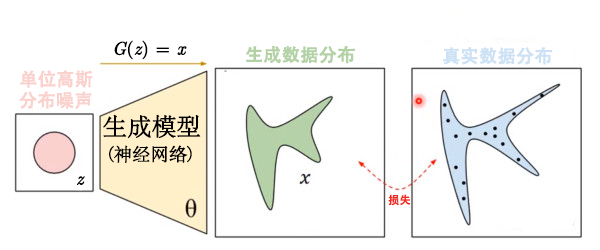
\includegraphics[width=0.8\textwidth]
    {figures/ganprograss.png}\\
    \caption{一般GAN网络模型结构}
    \label{fig:GAN}
  \end{figure}

\subsection{衍生模型分类与特点}
目前对抗生成网络的衍生模型众多,其优化方式大抵由两个大方向衍生而来。一个方向是由损失函数的改变来优化GAN模型的效果,另一个方向则是从模型使用的角度来优化GAN模型的效果。在表~\ref{tab:1.1}中,列举了一些最为常见的GAN模型衍生模型。

\begin{table}[!htb]
    \centering
    \caption{}
    \label{tab:1.1}
    \begin{tabular}{cccc}
        \toprule
        从损失函数角度&\multicolumn{3}{c}{从模型应用角度提出的优化GAN模型}\\
        \cline{2-4}
        提出的优化GAN模型\upcite{fgans}&网络构架角度\upcite{mirza2014conditional}&编码器角度&其他角度改进\\
        \hline
        \multirow{5}{0.3\textwidth}{Least Square GANs, Loss-Sensitive GAN, Fisher GAN, WGAN, WGAN-GP, WGAN-LP, f-GANs\upcite, DRAGAN等}&\multirow{5}{0.19\textwidth}{CGAN, DCGAN, InfoGAN, StackGAN\upcite{zhang2017stackgan}, AL-GAN等}&\multirow{5}{0.19\textwidth}{BEGAN, VAE-GAN, tDCGAN, BiGAN,文献中的算法\upcite{编码器GAN1, 编码器GAN3, 编码器GAN2}等}&\multirow{5}{0.19\textwidth}{LAPGAN, ESRGAN, SRGAN, 3D-GAN, MGAN等}\\ \\ \\ \\ \\
        \bottomrule
    \end{tabular}
\end{table}

图像生成的模型与基于网络构架优化的GAN网络模型最为贴合,本文设计使用StackGAN作为基础,并针对相关实现进行优化。

\subsection{StackGAN及其衍生模型}
Han Zhang et al.在2017年提出了StackGAN模型,创新性地提出了基于栈的对抗式生成网络模型从文本生成图片的方法。

StackGAN和CGAN同属于优化了GAN网络的构架结构的一类GAN模型的分支。其中,StackGAN是对相对朴素的CGAN模型的优化。

\subsubsection{从CGAN到StackGAN}
条件对抗生成网络(Conditional GAN, CGAN)是Mirza\upcite{mirza2014conditional}于2014年提出的,如公式\eqref{eq:CGAN}表述,对生成模型和判别模型输入文本信息作为条件,使用了一个隐藏层的全联通网络(MLP)结构,实现了通过文字标签生成图像的功能。
\begin{equation}
  \min_G\max_DV(G,D)=\mathbb{E}_{x\sim P_{data(x)}}[\lg D(x_i\mid y)]+\mathbb{E}_{x\sim P_G(z)}\lg [(1−D(G(z_i\mid y)))]
  \label{eq:CGAN}
\end{equation}

\begin{figure}[t]
  \centering
  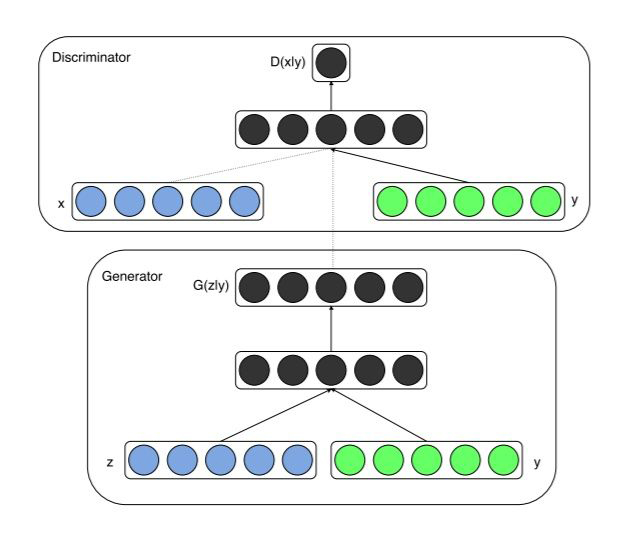
\includegraphics[width=0.5\textwidth]{figures/cgan.jpg}\\
  \caption{CGAN构架示意\upcite{mirza2014conditional}}
  \label{fig:CGAN}
\end{figure}

\begin{figure*}[t] 
  \centering 
  \begin{minipage}[c]{0.6\textwidth} 
    \begin{minipage}[c]{0.9\textwidth}
      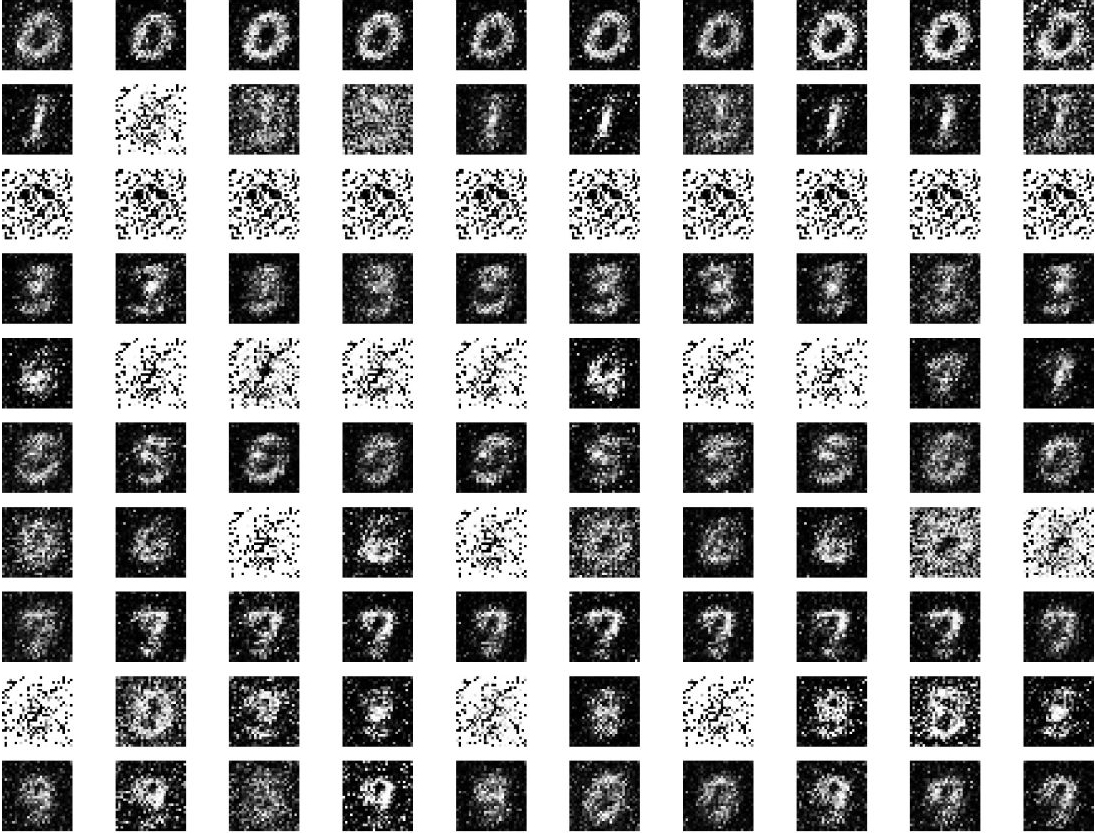
\includegraphics[width=0.45\textwidth]{figures/cgan手写数字1.jpg}\hspace{0.5em}
      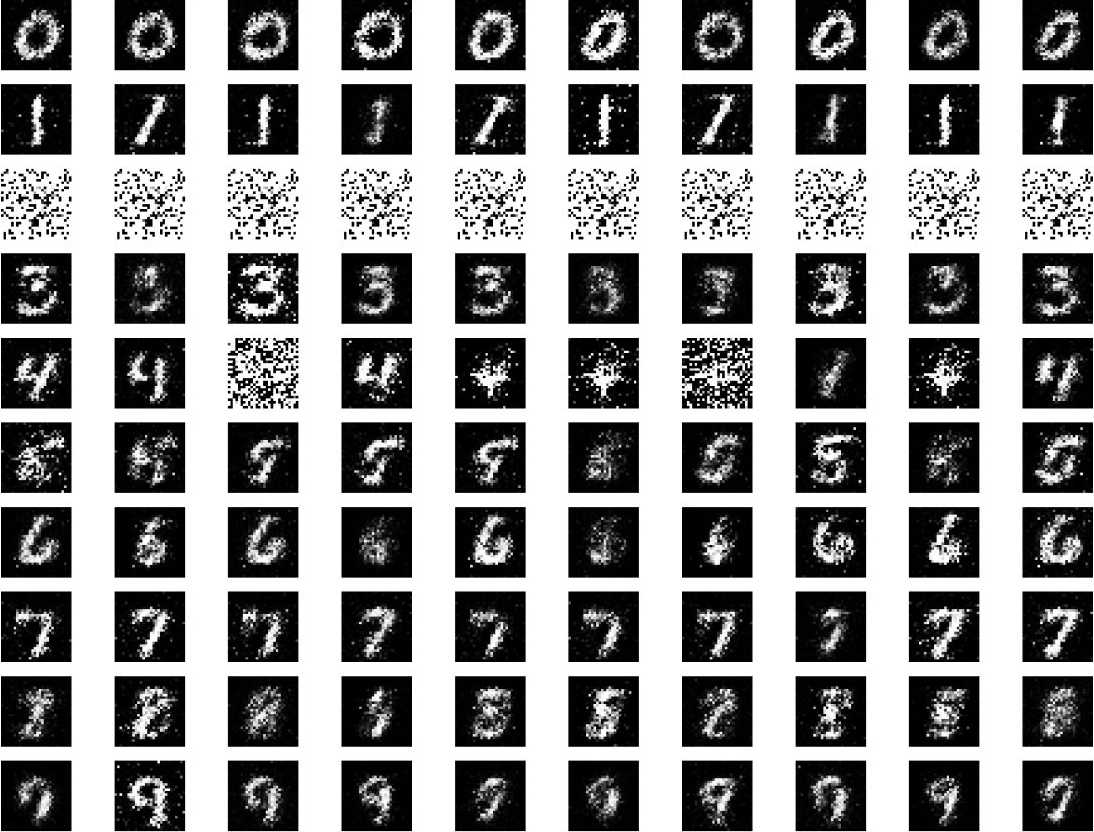
\includegraphics[width=0.45\textwidth]{figures/cgan手写数字2.jpg}
    \end{minipage} 
    \hfill \\ \vspace{0.5em}\\
    \begin{minipage}[c]{0.9\textwidth}
      \hspace{0.22em}
      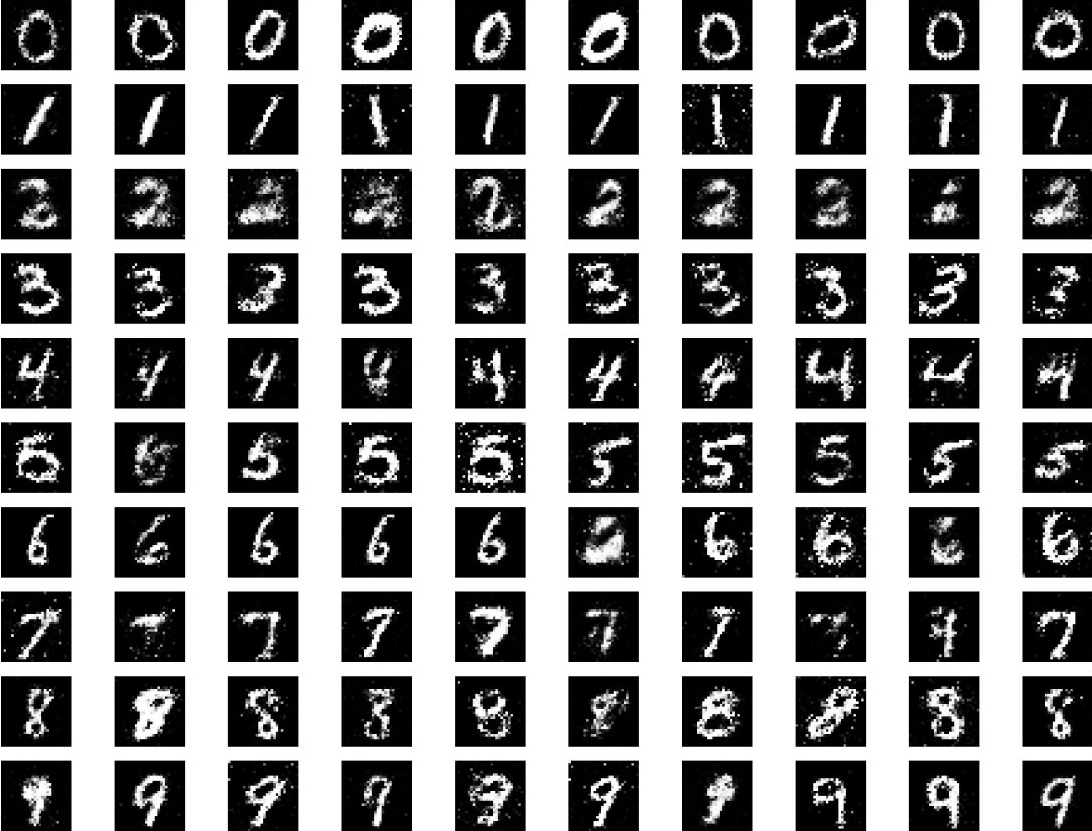
\includegraphics[width=0.45\textwidth]{figures/cgan手写数字3.jpg}\hspace{0.5em}
      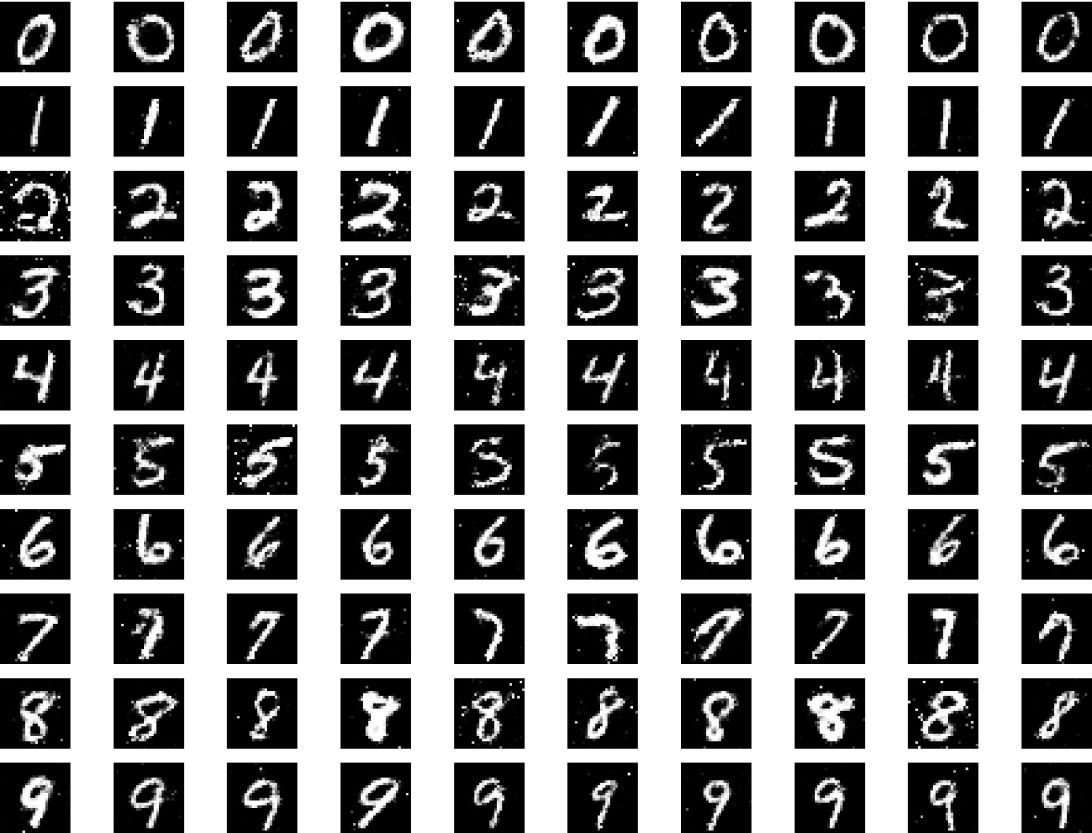
\includegraphics[width=0.45\textwidth]{figures/cgan手写数字.jpg}
    \end{minipage}
  \caption{CGAN生成手写数字\upcite{mirza2014conditional}(分别经历1、10、100、1000 个epoch后的结果)} %,zhihucgan
  \label{fig:cgan手写数字} 
  \end{minipage}
  \hfill 
  \begin{minipage}[c]{0.3\textwidth} 
  \centering%该小页居中排放图片 
  %\vspace{2em}
  \centerline{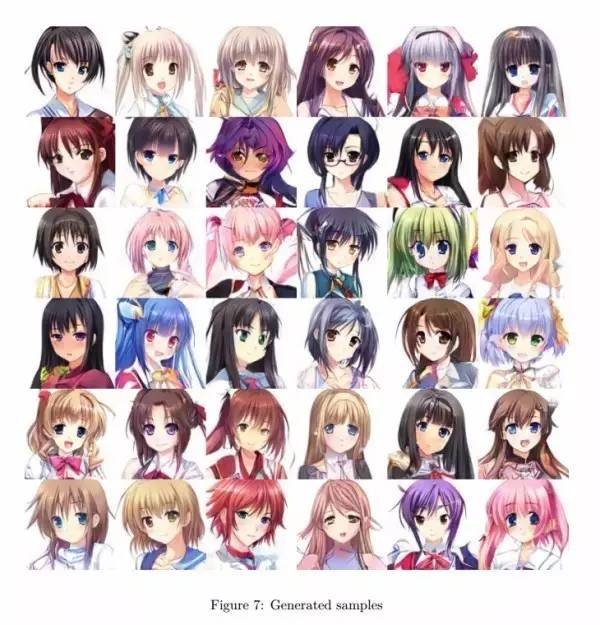
\includegraphics[width=1\textwidth]{figures/moegirl.jpg}}
  %\vspace{2em}
  \caption{CGAN生成二次元头像\upcite{2017comike}} 
  \label{fig:萌娘} 
  \end{minipage} 
  \end{figure*}

但是,CGAN的模型结构简单,效果差,收敛速度慢。在CGAN中,将文本作为条件输入生成器和判别器来训练两个模型生成和判别图像。如图~\ref{fig:cgan手写数字}和图~\ref{fig:萌娘}所示,及时CGAN应用广且有趣,但图像较小,质量不高。最基础的CGAN算法只能生成$64\times64$像素的图片,经过后来的改进,也只能将图片质量提升到$128\times128$像素。

  为了解决这一问题,Han Zhang\upcite{zhang2017stackgan}在2016年提出了StackGAN模型,使用基于栈的结构,分两步进行训练。
  
  如图~\ref{fig:StackGAN}所示,第一步先训练模型使模型生成$64\times 64$像素的图片,训练出的模型只能输出像素低、形状有所扭曲的图片。第一次训练的时候并不使用转化为向量的文字直接作为输入,因为这一向量为1024维,过于稀疏,不利于深度的训练。在经历一次FC以后进行输入,这样可以增强表现。
  第一阶段训练的损失函数为式\eqref{stackgan_loss1}所示。
  第二次训练并不增加噪声输入,经过多轮残差网络迭代,
  %残差网络可以实现梯度的跨层传播,解决深度网络里面梯度消失的问题
  模型修正一轮训练生成图片的错误,并且在图像中添加细节,生成$256\times256$像素的“高清图片”。
  第二阶段训练的损失函数如式\eqref{stackgan_loss2}所示。
  \begin{equation}
    \begin{aligned}
      &&\mathcal{L}_{D_0} = & \mathbb{E}_{(I_0,t) \sim P_{data}}[\lg D_0 (I_0,\varphi_t)] \\ && &+\mathbb{E}_{z\sim P_z,t \sim P_{data}}[\lg (1-D_0(G_0(z, \hat{c}_0 ),\varphi_t))],
      \\
      &&\mathcal{L}_{G_0} = & \mathbb{E}_{z\sim P_z,t \sim P_{data}}[\lg (1-D_0(G_0(z, \hat{c}_0 ),\varphi_t))]  \\ && &+\lambda D_{KL}(\mathcal{N}(\mu_0(\varphi_t),\Sigma_0(\varphi_t))\parallel \mathcal{N}(0,I))
      \end{aligned}
    \label{stackgan_loss1}
  \end{equation}
  \begin{equation}
    \begin{aligned}
      &&\mathcal{L}_{D} = & \mathbb{E}_{(I,t) \sim P_{data}}[\lg D (I,\varphi_t)] \\ && &+\mathbb{E}_{s_0\sim P_{G_0},t \sim P_{data}}[\lg (1-D(G(s_0, \hat{c} ),\varphi_t))],
      \\
      &&\mathcal{L}_{G} = & \mathbb{E}_{s_0\sim P_{G_0},t \sim P_{data}}[\lg (1-D(G(s_0, \hat{c} ),\varphi_t))]  \\ && &+\lambda D_{KL}(\mathcal{N}(\mu(\varphi_t),\Sigma(\varphi_t))\parallel \mathcal{N}(0,I))
      \end{aligned}
    \label{stackgan_loss2}
  \end{equation}
    
  \begin{figure}[!htb]
    \centering
    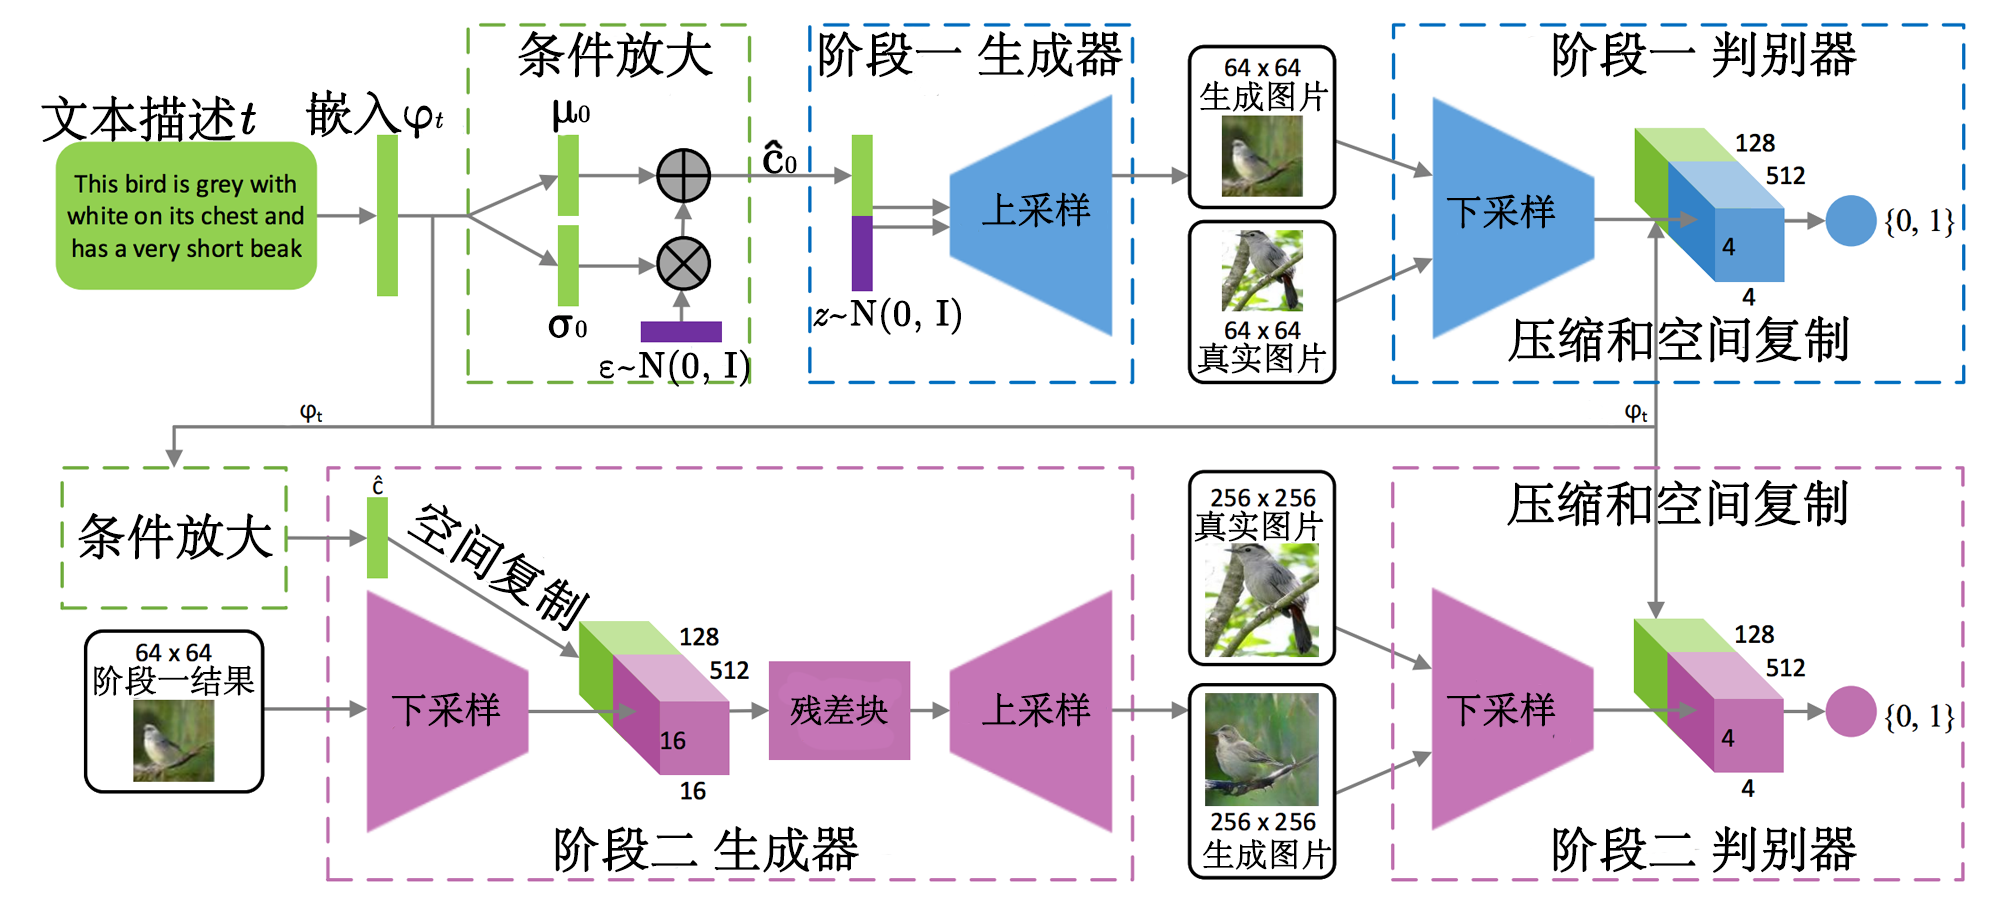
\includegraphics[width=0.95\textwidth]{figures/StackGAN.png}\\
    \caption{StackGAN构架示意}
    \label{fig:StackGAN}
  \end{figure}


  StackGAN模型相比较于CGAN模型,可以生成更高清的图片,而且结构更为真实。

\subsubsection{对StackGAN的进一步优化与运用}
同一课题组紧接着提出了StackGAN++\upcite{zhang2018stackgan++},对原有算法进一步进行了优化。StackGAN++模型也叫做StackGAN\_v2,对之前的StackGAN模型主要有三点改进。第一,改为采取树状结构作为输入,通过不同的生成器来生成不同尺寸的图片,多层次叠加形成了有位置关系的“假图片”,即混合图层叠加图片;第二,额外引入了非条件性的损失,直接将服从正态分布的损失$z$叠加在最后生成的“假图片”上;第三,引入了色彩限制,限制了最终“假图片”的色彩信息分布。

李飞飞课题组的Johnson\upcite{Johnson_2018}在StackGAN模型之上,提出了自己的优化。

该方法主要有三个特点:第一是有一个处理场景图的方法,第二是确保了生成的图像中个物体正确,且位置关系合理。第三是确保了生成图像的质量比较好。
其具体技术路线将在下一章进行推导和研究。

\section{本章小结}
本章主要总结了本次技术方案的前置技术,包括神经网络中的LSTM-RNN长短期记忆循环神经网络模型和StackGAN模型及其相关技术。LSTM-RNN模型是一种相对稳定、收敛,可以一定程度上避免梯度消失的深度学习模型,主要为下一章实现图片标注方法的技术做好铺垫。StackGAN及其升级版本是Han Zhang及其他科研人员2016年其后提出的一系列理论,本章内简要阐释了它的背景、原理和与后续技术的比较,决定使用李飞飞课题组的场景图像生成方法作为实现的理论依据,也为下一章自然语言生成图片的方法做好了前置说明。
  % Chapter 3

\chapter{方案设计}

\section{概要}
设计要求是:用户输入一张图片后,可以得到相应的标注语句,了解图片语义;在用户输入一句话的时候,可以得到描述这一句话的图片,直观“感受”文字。

软件设计主界面使用python的tkinter包来制作。python是一个跨平台语言,用python制作方便产品在不同平台使用。界面中应当可以选择调动两个功能,分别是图片翻译为自然语言和语句翻译为图片。两个功能分别提前训练出成品模型,通过主界面按钮内嵌入的方法,调用对应模型进行计算。

\section{软件模型}
软件分为三个部分,第一部分是软件界面,需要实现简洁明了的操作功能,方便使用。

第二部分是图片标注功能。实现这一功能的模型通过image caption的模型进行训练,算法参照蒙特利尔大学Kevin Xu\upcite{xu2015show}提出的模型进行实现,并经过基于一个或多个数据集进行多个epoch的训练,比较选出表现较好的模型,嵌入到应用中使用。

第三部分是文本生成图片功能。实现这一功能的模型通过一个特殊的GAN模型进行训练,并且要加入后期图片处理算法,以骗过判别器并使其更加真实。这一模型参照卡耐基-梅隆大学Justin Johnson\upcite{Johnson_2018}提出的基于场景双GAN模型配合进行实现,并经过合适的数据集训练,得到表现较好的模型,嵌入到应用当中使用。

\section{变量符号与定义}
文中使用集合如下:
\begin{enumerate}[fullwidth,itemindent=2em,label=\arabic*.]
    \item $O$代表物品(object)的集合;
    \item $C$代表物品目录(catagory)的集合;
    \item $R$代表关系(relationship)的集合;
    \item $E$代表物品-关系-物品组成的边(edge)的集合。
\end{enumerate}

文中脚标定义如下:
\begin{enumerate}[fullwidth,itemindent=2em,label=\arabic*.]
    \item ${}_t$代表LSTM模型中的时序,${}_t$为当前时序,而${}_{t-1}$或${}_{t+1}$为前一或后一时序;
    \item $_f$代表任一函数(使用$f$指代)代入当前操作或模型;
    \item $v_i$在第二个算法中,代表GCN当前层级的节点编号,因为不讨论跨多层关系,所以脚标中不增加时序信息。
\end{enumerate}

文中小写字母对象定义如下:
\begin{enumerate}[fullwidth,itemindent=2em,label=\arabic*.]
    \item $s$指代集合$S$中的元素,其中$S$指代任一集合,如物品集合$O$等,他们通常和集合一起出现;
    \item $c$代表LSTM模型中的细胞(cell),记录细胞当前状态;
    \item $i$代表LSTM模型中的输入门(input),执行LSTM模型中的输入操作;
    \item $o$代表LSTM模型中的输出门(output),执行LSTM模型中的输入操作;
    \item $f$代表LSTM模型中的遗忘门(forget),选择LSTM细胞的部分状态丢失;
    \item $z$代表生成模型中为了骗过判别器、降低生成图片锐度增加的噪声。
\end{enumerate}

文中主要函数定义如下:
\begin{enumerate}[fullwidth,itemindent=2em,label=\arabic*.]
    \item $\phi$代表注意力机制;
    \item $\mathcal{L}$函数代表GAN模型中用作训练目标函数的损失函数;
    \item $f(S,z)$代表自然语言生成图像算法中的目标函数。
\end{enumerate}

\section{软件界面设计}
\subsection{软件例图}
对于预期的软件效果,我制作了原型图(图~\ref{fig:UIproto})进行示意。图中,应当出现英文的地方用英文示意,应当出现路径的地方用路径示意,而应当出现中文的地方和说明文字使用中文表述。
\begin{figure}[!htb]
    \centering
    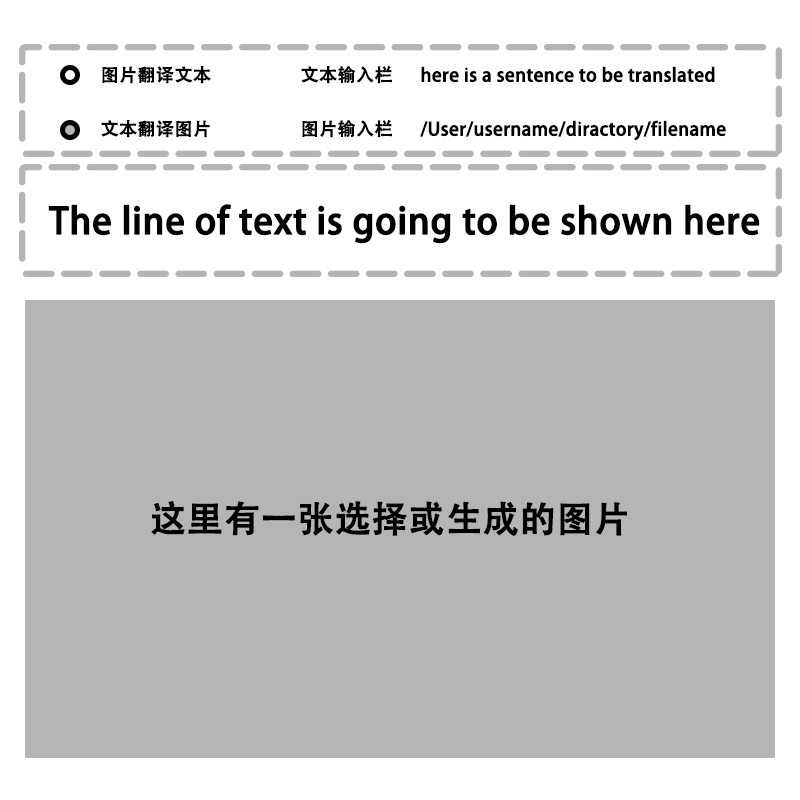
\includegraphics[width=0.8\textwidth]{figures/界面原型图.png}
    \caption{软件界面原型图}
    \label{fig:UIproto}
  \end{figure}

  其中,界面上方由一组两个单选选项的选择栏和两个数据输入栏组成。选项栏的作用是选择当前需要实现的功能,由“图片翻译语义”和“文本翻译图片”两个选项组成;数据输入栏分别是一个文本输入栏和一个文件选择栏,分别对应着文本和图片的输入选择。

  其下是一个明显的按钮,突出的设计可以让用户能轻易明白操作方法,也让用户更有仪式感,能感受到这一操作的划时代意义。

  最下方的大区域是输出区域,根据功能的不同可以输出不同的内容。在选择图像翻译语义功能时,会输出一句话,这一行文字和图片将一起显示,方便对比观察;在选择语义生成图像选项时,将输出生成的图片和原语句,也是为了方便用户观察与分享,表意清晰。

\subsection{软件开发模型}
对开发设计软件的过程,我选用了编码-修改模型\upcite{pressman2005software}。如图~\ref{fig:codenfix}所示,在这一模型中不进行计划与建模,先进行编码,调整至用户满意时,发布运行,在出现问题与更新时维护,直到软件生命周期结束为止。

本次软件设计开发的过程是要独立接触一个不熟悉的领域,对于开发者来说不易估计编码需要的时间。深度学习对初学者来说有一个难点:环境安装中很多细节难以把控;并且深度学习的学习过程需要使用多块显卡进行天级时长的训练过程,才可以得到结果。基于上述理由,我可以推测算法的实现需要比较长的时间,并且可能一次训练出的算法达不到理想的状态,需要调整模型、重复训练。

\begin{figure}[!htb]
    \centering
    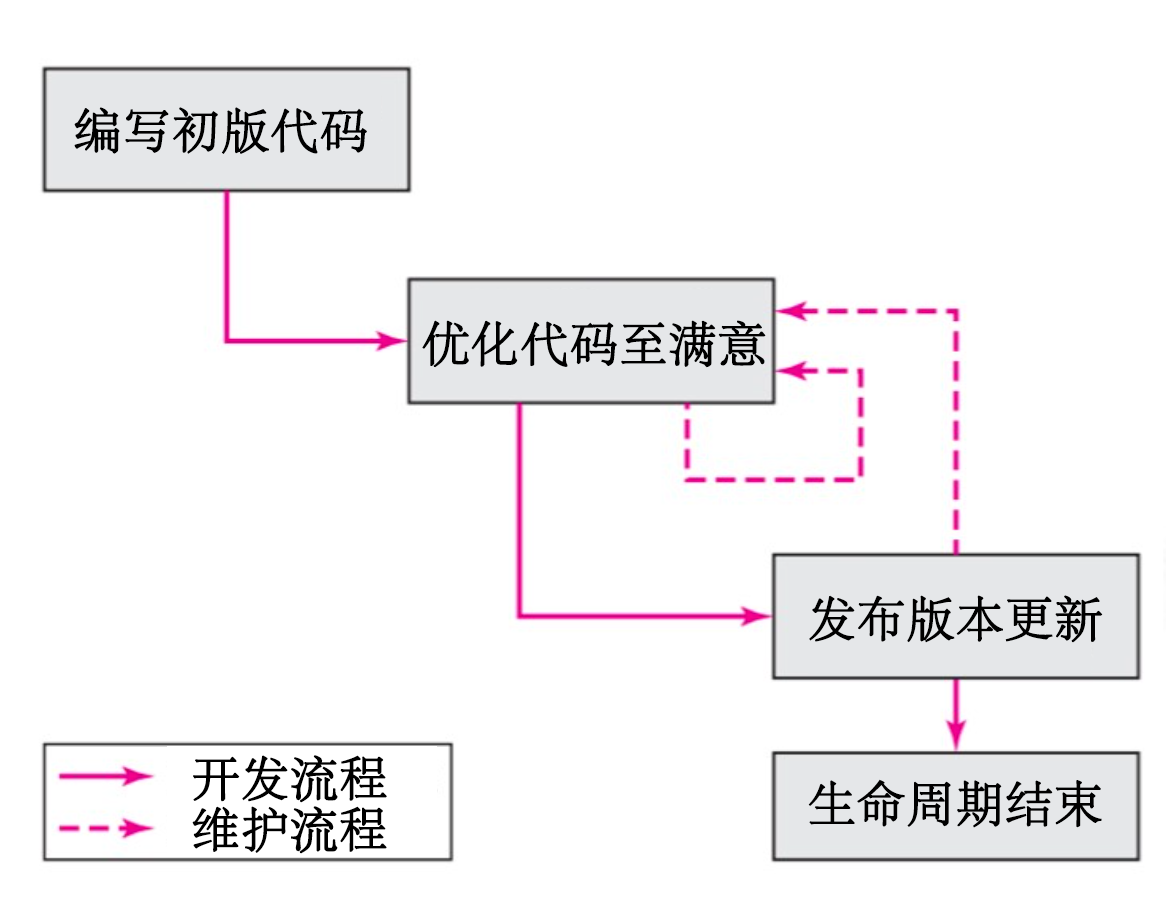
\includegraphics[width=0.6\textwidth]{figures/codeandfix.png}
    \caption{编码-修改模型的基本结构}
    \label{fig:codenfix}
\end{figure}

在设计的过程中,对我来说的难点的确是环境安装部分。需要的新虚拟容器因为电脑上旧有的项目擅自修改了环境变量,需要重新安装、整理环境,并且安装合适版本的环境,搭配当前系统,对开源项目进行修改、复现,并在此基础上进行改进。

另外,本软件的模型相对比较简单,是用户界面-调用模型的两层结构,难点在于模型的建立和调整。所以本设计非常适合使用编码-修改模型进行开发。

\section{软件功能设计}
功能部分分为图片标注功能以及文字生成图像功能,两个功能我使用了两个结构相对复杂的深度学习模型组合构架的算法,将在下面具体介绍。
 
\subsection{图片标注方法}
\subsubsection{算法整体模型}
在这一模型中,要使用LSTM模型进行训练,训练出的模型放在主函数的调用函数中,实现图片翻译为自然语言的功能。

这一模型主要流程由四步组成。

\begin{enumerate}[fullwidth,itemindent=2em,label=\arabic*.]
    \item 在模型中输入图片,作为输入信息;
    \item 由卷积神经网络提取图片信息,形成图片特征信息(即后文编码步骤);
    \item 由注意力机制(attention)对所提取的图片特征信息进行处理,加强或抑制部分区域,作为后续输入LSTM的输入信息——在不同时刻,注意力信号会受到上一次LSTM的输出信息的影响,即注意力信号作为LSTM神经元细胞的状态,受到输出词语的影响而改变(这也是后文的解码部分);
    \item LSTM最终输出文本,形成最后的结果。
\end{enumerate}

\subsubsection{编码部分}
第一步,要对训练集中的标注编码,形成特征向量。词典中已经预先确定了$K$个词语,对于每一行标注$y_i$,可以将其通过词典序号,将句子映射成输入向量,每一个元素的位置意义是序号,即图片相关的类别,数字则是关联度。编码之后生成向量$\textbf{y}_i$,一起构成输入矩阵。
$$y = {\textbf{y}_1, \textbf{y}_2, ..., \textbf{y}_C}, \textbf{y}_i\in \mathbb{R}^K$$

第二步,对图片编码。使用一个卷积神经网络(Convolutional Neural Network, CNN)对图片的特征进行提取,从而形成图片编码。编码好的图片,后续会作为注释向量$\textbf{a}$使用。
$$a = \{\textbf{a}_1, \textbf{a}_2, ... , \textbf{a}_L\}, \textbf{a}_i \in \mathcal{R}^D$$

\subsubsection{解码部分}
解码部分使用的技术是LSTM,即长短期记忆模型。解码后生成的是标注文本,在预测最后一个词的时候,需要背景向量、前一时刻的隐藏层向量、前一时刻的词。这一部分实用的LSTM模型结构,由图示意出。
\begin{figure}[!htbp]
    \centering
    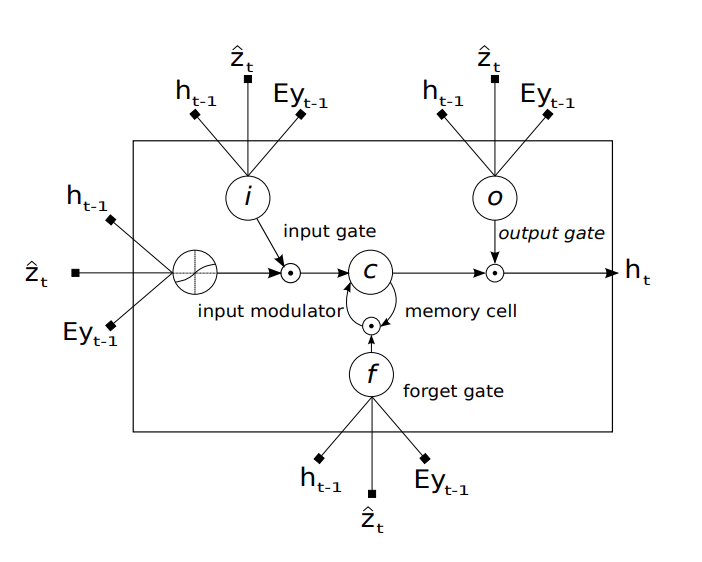
\includegraphics[width=0.8\textwidth]{figures/lstm_token.png}
    \caption{解码LSTM神经元细胞模型结构图}
    \label{fig:lstm_tokenize}
\end{figure}

背景向量$\hat{z}_t$由注意力机制函数和图片注释向量计算得出,并且与时序$t$有关,随时序推进而变化。相当于是有选择地传输图片注释向量中的信息,是图片信息的动态表达。

确定一个注意力机制函数$\phi$来计算$t$时刻的背景向量$\hat{z}_t$。对于输入的图片注释信息,为了推测这一位置是否是正确的注意力集中点,在式\eqref{eq:归一a}中定义一个可以归一化的参数$\alpha_{t,i}$来表示在$t$时刻,位置$i$是正确关注点的置信度。
\begin{equation}
    e_{t,i}=f_{att}(\textbf{a}_i,\textbf{h}_t)
\end{equation}
\begin{equation}
    \label{eq:归一a}
    \alpha_{t,i}=\frac{\exp e_{t,i}}{\sum_{k=1}^{L}\exp e_{t,k}}
\end{equation}

计算置信度时需要用到$f_{att}$函数,这一函数定义为一个“硬”机会注意力机制函数。
这一机会注意力机制的“软”版本由Bahdanau\upcite{bahdanau2014neural}提出,仿照这个机制可以提出硬版本函数。

现在定义$s_t$为模型为了生成第$t$个单词所选择的注意力区域。其中,$s_t$的第$i$项是开关函数,此项置1时,当前模型生成打你是第i个单词。
现设定多次伯努利分布的参数${\alpha_i}$,将背景向量视为随机事件,则有:
\begin{equation}
    p(s_{t,i} = 1|s_{j<t}, \textbf{a}) = \alpha_{t,i}
\end{equation}

计算出权重之后,即可使用注意力机制函数计算出背景向量$\hat{z}_t$:
\begin{equation}
    \label{eq:bgvector}
    \hat{z}_t=\phi(\textbf{a}_i,\alpha_i)
\end{equation}
\begin{equation}
    \hat{z}_t = \sum_i s_{t,i}\textbf{a}_i
\end{equation}
一个“软”估计得算法即如式\eqref{eq:softatt}的方法计算出。但是,还可以提出一种“硬”估计的
\begin{equation}
    \begin{aligned}
        &&\phi(\{\textbf{a}_i\},\{\alpha_i\})&= \mathbb{E}_{p(s_t\mid a)} [\hat{z}_t] \\
        && & =\sum_{i=1}^L \alpha_{t,i} \cdot \textbf{a}_i \\
    \end{aligned}
    \label{eq:softatt}
\end{equation}

现在定义一个概率的对数函数,计为$L_s$,作为模型的优化目标;对于训练的目标参数$W$,$L_s$函数就是优化目标。则可以推导得其下界为式\eqref{eq:hard1}所示,从而得到最终训练梯度为式\eqref{eq:lstmtar}
\begin{equation}
    \begin{aligned}
        && L_s &= \sum_s p(s, \textbf{a}) \log p(\textbf{y}\mid {s }, \textbf{a} ) \\
        && & \le \log \sum_sp(s, \textbf{a}) p(\textbf{y}\mid {s }, \textbf{a} ) \\
        && & = \log p(\textbf{y}, \textbf{a})
    \end{aligned}
    \label{eq:hard1}
\end{equation}
\begin{equation}
    \frac{\partial L_s}{\partial W} = \sum_s p(s \mid a) [\frac{\partial \log p(\textbf{y}\mid {s }, \textbf{a} )}{\partial W} + \log p(\textbf{y}\mid {s }, \textbf{a} ) \frac{\partial \log p(\textbf{y}, \textbf{a})}{\partial W} ]
    \label{eq:lstmtar}
\end{equation}

其中有
\begin{equation}
    \tilde{s}_t \sim Multinoulli_L({\alpha_i})
    \label{eq:stdistribute}
\end{equation}

则
\begin{equation}
    \frac{\partial L_s}{\partial W} \approx \frac{1}{N} \sum_{i=1}^{n} [\frac{\partial \log p(\textbf{y}\mid \tilde{s}^n, \textbf{a} )}{\partial W} + \log p(\tilde{s}^n \mid \textbf{a} ) \frac{\partial \log p(\textbf{y}, \textbf{a})}{\partial W} ]
    \label{eq:lstmtar2}
\end{equation}

这里的函数$\phi$是利用了“软”确定注意力机制(Deterministic “Soft” Attention),这一机制算法可以稍为简易地作出注意力正确位置的判断,可以作出计算,用于判断下一个词的注意力位置;并且,这个函数的目的是计算注意力,而非前文从提取注意力。可以将$\hat{z}_t$的期望值$\mathbb{E} [\hat{z}_t]$作为其取值,带入计算,即设定$\phi$函数为式\eqref{eq:softatt}中的计算方法。

从式\eqref{eq:lstmtar}中,可以看出优化函数$L_s$由基于蒙特卡罗方法多次采样逼近梯度的方式,对式\eqref{eq:stdistribute}遵从多次伯努力分布的注意力区域位置进行采样,测算优化函数。在这个时序数据中,为了消除,使用滑动平均基线的方法\upcite{10.5555/2074022.2074088},令基线的对数更新比例如式\eqref{eq:baseline}所示。
\begin{equation}
    \label{eq:baseline}
    b_k = 0.9 \times b_{k-1} + 0.1 \times \log p(\textbf{y} \mid \tilde{s}_k, a)
\end{equation}

最终得到的“硬”注意力函数如式\eqref{eq:hard3}所示。
\begin{equation}
    \frac{\partial L_s}{\partial W} \approx \frac{1}{N} \sum_{i=1}^N\left[\frac{\partial \log p(\textbf{y}\mid \tilde{s}^n,\textbf{a})}{\partial W} + \lambda_r[]\log p(\textbf{y}\mid \tilde{s}^n,\textbf{a})-b] \frac{\partial \log p(\tilde{s}^n \mid \textbf{a})}{\partial W} +\lambda_e\frac{\partial H[\tilde{s}^n]}{\partial W}\right]
    \label{eq:hard3}
\end{equation}

将其代回式\eqref{eq:bgvector}中的$\phi$函数,即可得出${\textbf{a}_i}$由“硬”选择注意力集中位置的参数${\alpha_i}$加权后的取样结果。

解决了背景向量的问题,可以开始训练LSTM模型了。对于这个模型,需要进行初始化,确定其中图~\ref{fig:lstm_tokenize}标注的传入隐状态$h_0$及其内部初始环境$c_0$。取标注向量的平均,作为初始的状态,进行操作。即:
$$\textbf{c}_0 = f_{init,c}\left(\frac{1}{L}\sum_{i=1}{L}\textbf{a}_i\right)$$
$$\textbf{h}_0 = f_{init,c}\left(\frac{1}{L}\sum_{i=1}{L}\textbf{a}_i\right)$$
%\subsubsection{代码实现模块}

\subsection{自然语言生成图片方法}
这一模型主要是用通过场景生成图像的GAN模型来训练,得到的模型放在主函数的调用函数中,实现自然语言生成图片的功能。

\subsubsection{图片生成模型}
生成图片的总体的算法流程如算法~\ref{algo:sg2im-all}所示,分为三个大步骤:GCN确定场景布局,确定图像边框布局,级联优化网络(Cascade Refinement Network)\upcite{chen2017photographic}。

\begin{algorithm}[H]
    \setstretch{1.5} % 代码间行距设定
    \SetAlgoLined
    \vspace{2em}
    \algorithmicrequire 自然语言短句$S$,噪声$z$\\
    \algorithmicensure 生成图片$\hat{I} = f(G,z)$\\
    %\Function{a}{b}
    $O,E \gets $提取(物品)元素和(位置)关系$($生成语义树$(S))$\;
    $G \gets $构成物品关系图$(O,E)$\;
    $\textbf{Layout} \gets $GCN$(G)$\;
    $I \gets Generate(Layout)$ \;
    $\hat{I} \gets CRN(I)$\;
    %\EndFunction
    \caption{图片生成方法}
    \label{algo:sg2im-all}
\end{algorithm}

\vspace{2em}
第一步的图卷积网络(GCN)需要输入场景关系图,它是由自然语言经过简单处理后得到的。场景关系图满足下列条件:
$$O={o_1,...,o_n},o_i \in C$$
$$E \subseteq O \times R \times O =\{(o_i,r_{ij},o_j)\mid i,j \in \mathbb{N}^\star\}, r \in R$$

图卷积网络可以沿着场景图的关系(边)$e_i$,计算出图中各个物体$o_i$的嵌入向量$ \textbf{v}_i$。其单层局部结构如图~\ref{fig:gcn}所示,这张图示意了图卷积网络的每一层之间,向量如何更新迭代。

\begin{figure}[!htb]
    \centering
    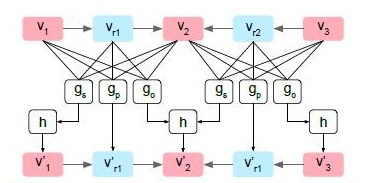
\includegraphics[width=0.9\textwidth]{figures/gcn.png}
    \caption{图卷积神经网络(GCN)单层结构图}
    \label{fig:gcn}
\end{figure}
图~\ref{fig:gcn}中$v_i$代表物体向量,而$v_{ri}$代表关系向量。其中涉及了三个物品$o_1, o_2, o_3$和两组关系$(o_1,r_1,o_2), (o_2,r_2,o_3)$。这些向量需要经过三个函数,分别是$g_o, g_p, g_s$,其中$g_o, g_s$的值需要作为候选变量,参与到调和函数$h$中,最终决定更新后的物体向量。

关系向量的更新比较简单,它遵从式\eqref{eq:vrupdate}。
\begin{equation}
    v'_r = g_p(v_i,v_r,v_j)
    \label{eq:vrupdate}
\end{equation}

而图中的物体元素则更为复杂一些。要考虑每一个元素作为它参与的所有关系中的角色,而计算出它的更新向量。对于每一个物体向量$o_i$,它对应下列两个候选向量,供调和函数调用。其中$V_i^o $代表了所有$o_i$作为关系中被指向的点所在关系所生成的候选向量集合,反之 $V_i^s$ $o_i$代表了所有$o_i$作为关系中指向起点所在关系所生成的候选向量集合。
$$V_i^s = \{g_s(o_i, r, o_j)\mid (o_i, r, o_j)\in E\}$$
$$V_i^o = \{g_o(o_j, r, o_i)\mid (o_j, r, o_i)\in E\}$$

随后,我们可以通过式\eqref{eq:viupdate}中的调和函数更新物体向量$ v_i $。
\begin{equation}
    v'_i = h(V_i^s, V_i^o)
    \label{eq:viupdate}
\end{equation}

生成的图像还需要两个额外的生成模型进行优化,以得到平滑效果更好的生成图像。图像的平滑程度是评价生成图像质量的重要标准之一。

第一部分中,我们得到了最终得到了每个物体的高级特征表达向量(关系的特征表达向量主要作为隐藏值影响物体的特征向量计算)。在第二部分中,则需要测算每一个物体的框架位置。

对于上一环节得到的每一个物体的特征表达向量$\hat{v}_i$,我们分别将它传入蒙板回归网络(Mask Regression Network)和框回归网络(Box Regression Network),分别求出其在画布上的形状和位置。最终得到形状蒙板$\hat{m}$和$\hat{b}$:
$$\hat{m} \sim M \times M$$
$$\hat{b} = (x_0,y_0,x_1,y_1)$$

将$\hat{m} $和物体特征向量 $v_i $按照元素序逐一将值相乘,得到物体的形状与样式,再将其缩放,使其可以代入$\hat{b}$所规定的框架中,则可以得到这一物体的形状、位置与大小。

第三部分则是将在画布上的物体拼合,组成一幅新的“图像”。这个图像要求所有的元素都在其中对此,

\subsubsection{鉴别模型}
我们生成了两个鉴别网络模型,用作与前述生成模型进行对抗。

第一个判别器$D_{img}$是对整个$f$ 函数结果,即生成图片$\hat{I}$进行判别。这个判别器的损失函数是:
\begin{equation}
    \mathcal{L}_{D_{img}} = \mathbb{E}_{x\sim p_{real}} [\log D(x)] + \mathbb{E}_{x\sim p_{fake}} [1-D(x)]
    \label{eq:lossdimg}
\end{equation}
其中,$x\sim p_{real}$指训练集中提供的真实图片$I$,而$x\sim p_{fake}$则是指生成图片$\hat{I}=f(g)$。生成模型函数$f$的训练目标是最小化判别器得出的$\mathcal{L}_{D_{img}}$值。

$f, \mathcal{L}_{D_{img}}$函数组成的GAN网络模型,保证了图片整体的真实性和平滑性,与\cite{isola2017image}中的判别器性质类似。

当然,在生成模型第二部分生成的物体图片要单独进行训练,这就需要一个使用另一个判别器${D_{obj}}$来进行对每个物体的图像判别。但是物体的图像大小可能会与原图不相同,但这是不影响图片生成效果的,所以在判别之前需要用双线性插值\upcite{双线性插值}的方法将图片变换处理为相同的大小,以减小大小对判别带来的过拟合。 

除此之外,判别器还要做一项特殊的工作。与以往的GAN网络不同,它是一道保险装置,希望再不输入物体类别,仅输入生成图像时,将物体判别为正确的分类。在这一方面,判别器和生成器都希望正确类别的置信度尽量高,以保证其在\cite{odena2017conditional}中提到的判别标准(Auxiliary Classifier)中的可识别性。

经过以上恰当的双GAN模型训练与保险机制,可以得到可用的图片生成器$f$。

\section{本章小结}
本章具体地介绍了这一设计中所包含的设计细节及其理论依据,并确定了软件构架的结构,为完成代码构建和实验设计打下了基础。

本章中,确定了以python语言的tkinter库来写界面,保证界面简单简介易懂;用CNN和LSTM技术,基于注意力的方法,通过编码-解码的流程来完成图片标注功能;用基于位置场景的方法,由GNN和两个判别器构成的GAN模型来分步生成图片,最后生成合成图片的方法来实现由文本生成图片的功能。

在下一章里,我会继续记述实验的过程及其表现。
%{\songti \bfseries 宋体加粗} {\textbf{English}}

%{\songti \itshape 宋体斜体} {\textit{English}}

%%%{\songti \bfseries \itshape 宋体粗斜体} {\textbf{\textit{English}}}

%\section{编译}
%本模板必须使用XeLaTeX + BibTeX编译,否则会直接报错。 本模板支持多个平台,结合sublime/vscode/overleaf都可以使用。
  % Chapter 4

\chapter{实验与分析}
\section{实验环境}
\subsection{模型训练环境}
服务器环境,操作系统为
Ubuntu 16.04.6 LTS (GNU/Linux 4.4.0-142-generic x86\_64),使用命令行ssh工具登入。

内存64GB,搭配显卡2080 Ti 四块,由于资源分配原因本设计中实验使用两块。

使用anaconda 创建虚拟环境,为算法各自安装需要的依赖包与训练环境。
\subsection{软件样本运行环境}
Macbook Pro电脑 15.6寸屏幕版,mid-15 release,A1398型号;
OS X 10.12(Serrina High)系统;
集成显卡,内存16G,没有特别要求。

\section{图片标注实验}
\subsection{模型代码}
模型主题使用了开源代码,由第三方代码作者完成,在Github网站上开源;同时我在其中做了修缮维护,保证了复现在当前版本的依赖包上和现在可以运行的系统里仍然可以运行。

原代码开发环境是python 2.7和tensorflow 0.14,由于目前科学计算使用的python以python3为主流,我将其修改维护至了python 3.6和tensorflow 1.14版本下可以运行的代码。

代码结构分为几个部分:主函数、基本模型类、训练算法。
\subsection{运行过程}
通过在论坛上调研、向专家咨询,我认为较少的数据会导致图片标注模型的效果减弱,会限定构图、限定主题、限定语汇,且识别精确度会很差。为此,我选用了MSCOCO数据集作为训练和测试集。对于这次实验,我先选择了最早的COCO2014数据集,作为试验,后来发现训练时间成本较长,决定使用COCO2014数据集下训练生成的模型作为应用模型。

这一算法的虚拟实验环境python版本为3.7,tensorflow版本为1.14.0,其中安装的依赖包有:numpy 1.17.2,OpenCV 4.1.1.26,NLTK 3.4.5,Pandas 0.25.1,Matplotlib 3.1.1,tqdm 4.36.1。
其中NLTK用作训练集中文字信息的分词处理,仅仅执行了nltk.download("punkt"),作为数据支撑,没有下载完整数据。

模型的训练在实验环境下使用4块NVIDIA 2080 Ti显卡,训练了233小时,执行了100个epoch,每一个epoch都遍历了训练集中的所有数据。

\subsection{遇到的主要问题与解决方法}
\subsubsection{数据传输问题}
服务器的物理地址在浙江大学,属于教育网的浙江位置,从我的工作地点到浙江大学校内当前跳转节点较多,使用RVPN进行连接后,数据传输速度上限是2.00Mbits/sec,所以传输一个总大小为19GiB以上的数据集,需要的时间为40000秒,相当于十余小时。另外,由于RVPN的连接不稳定,而scp命令传输文件不支持断点续传,所以经常出现文件损坏的现象。

经过多次尝试和实践,我采用分包的方式,将数据集化为1GiB到2GiB大小的压缩包,由scp命令逐一传输;同时使用完善、成熟的数据集,尽量最大化一次成功率。

\subsubsection{依赖包函数不兼容问题}
tensorflow在目前的稳定版本中,已经增加了很多新的借口,而1版本和0版本的接口,有一些已经取消了。即使我安装的是1版本的tensorflow环境,仍然有一些接口无法调用。经过调研,我使用了评价较高的tensorflow.compat.v1库,来实现变易出错的接口,解决了大部分问题。

\section{自然语言生成图片实验}
\subsection{模型代码}
模型使用了开源代码,由论文原作者完成,在Github网站上开源;同时我在其中微调,以适合我所需的数据集。

这一套代码的特点是,它含有一套下载数据集的bash代码,方便下载。这一套代码推荐在googleapis.com网站上直接使用wget命令下载数据,这样下载的数据传输速度比较稳定,可以正常下载使用数据。

代码主要包含一个模型运行的主函数、一个模型类和一个训练模型的方法。除此之外,以面向对象的思想对训练过程中的辨别器$D$等类、双线性插值、图片级联优化网络等方法都单独编码,然后加上工具方法的编码,构成了整个工程。

\subsection{运行过程}
运行中由于代码设计,只使用一块显卡进行训练。

因为显卡的设置问题,不可以同时使用同一块显卡即运行tensorflow模型,又训练pytorch模型,因为如果它们同时运行,不同的容器会导致驱动将所有显存都分配给tensorflow的任务,导致pytorch训练的模型无法正常运行。所以,需要等到上一模型训练完毕,再开始训练这一模型。或者,可以让它们在不同的显卡上运行。这在一定程度上影响了我的时间安排,导致我仅在VG数据集上运行了代码。

在VG数据集上,我使用了代码中编写的“强注意力生成”方法制作的生成模型,得到了一个可以从自然语言自动生成图片的模型。

\subsection{遇到的主要问题与解决方法}
这一模型更加的复杂,并且开源代码仅有pytorch版本的实现。按照要求,为了运行这段代码,需要安装python 3.5下的pytorch 0.4.0版本。但是,按照版本要求,在目前的cuda 版本为10.0的电脑中不可以安装这一版本的pytorch了,所以可以替代性地使用torch 1.0.0来运行程序。

在安装虚拟环境的时候,需要注意无论是anaconda官网默认源还是清华大学镜像源都难以链接,并正常下载完毕torch安装包,因为其大小高达700MB,在下载到一半的时候就常常会出现HTTP:200错误代码,导致下载中断。可以打出下列shell命令,将在官网下载好的whl文件安装在环境里。这里的包一定要符合环境下的python版本要求,不知道要求的可以在python shell中运行“wheel.pep425tags. get\_supported()”代码,查询wheel安装要求。

        \text{conda create venv env\_name}

        \text{conda activate env\_name}

        \text{pip\ install\ torch-x.x.x-cp3x-cp3xm-ostype.whl}

        \text{pip\ install\ torchvision}

\section{实验分析与总结}
\subsection{图片标注表现}
对图片标注的模型,我选取了三个模型作为对比,使用BLEU评分\upcite{papineni2002bleu}(Bilingual Evaluation Understudy)的方式进行评价。

BLEU评分是IBM出品的机器翻译评分标准,按照式\eqref{eq:bleu}的算法得出评分。这个评分是对一条翻译打出,后续数据中取平均得分。
\begin{equation}
    \begin{aligned}
        &&BLEU &= &BP \cdot \exp(\sum_{n=1}^N wn\log P_n) \\
        &&\text{其中, }BP&=
        &1 \hspace{9em}& c>r \\ && & &e^{1−r/c}\hspace{7.2em}&c<=r
    \end{aligned}
    \label{eq:bleu}
\end{equation}
式中$BP$即简短惩罚,即在句子短的时候降低评分。在本次评分中,不加入$BP$机制。

其中,我希望测试二十个epoch量级的训练是否可以支撑一个可用的模型,事实上19个epoch的模型经过个例测试,不能很好地生成注意力转移的机制,导致句子不够通顺,经常出现连续无意义重复关键词的现象。后来,我使用这一断点“214999.npy”(后称“断点模型”)继续训练,得到了100个epoch后生成的“289999.npy”(后称“强注意力模型”)模型。

另外,我引入了预训练的“弱注意力模型”的测试数据\upcite{xu2015show},作为对照,观察注意力机制对标注结果的影响,以选取最合适的模型,嵌入软件。对于上述三种模型,我使用nltk包中所带算法,使用1-4精度修正的四种评分进行评价,得到的结果如表所示。其中若关注模型和第二组强关注模型是文献\cite{xu2015show}中的结果。

\begin{table}[!htbp]
    \centering
    \caption{三种模型的BLEU评分}
    \label{tab:bleu}
    \begin{tabular}{cccccc}
        \toprule
        模型选择& BLEU-1 & BLEU-2& BLEU-3& BLEU-4 & METEOR\\
        \hline
        断点模型  & & & & &——\\
        弱关注模型 & 70.7\%&49.2\%&34.4\%&24.3\%&\textbf{23.90\%}\\
        强关注模型(我的训练)&70.3\% &\textbf{53.6\%}&\textbf{ 39.8\%}&\textbf{29.5\%}&——\\
        强关注模型(文中数据)& \textbf{71.8\%}&50.4\%&35.7\%&25.0\%&23.04\%\\
        \bottomrule
    \end{tabular}
\end{table}

可以看到,弱关注模型表现稍好于强关注模型,但是在原文中结论有所不同。因为我自己训练的数据可能因为环境不同表现有少许的差异,但是在同一环境下,强关注模型的训练结果更有利翻译的准确性。

\subsection{文本生成图像算法表现}
理解文本生成的图像涉及到图像标注这一不成熟且复杂度高的算法(正如前文工作所说),所以这一算法的表现不能使用BLEU评分来评价。对于这一图片是否被人理解,采用两种方法评价。

第一种是采用检查图片平滑性的一种评分\upcite{salimans2016improved}(Inspection Scores),作为量化的参考,检查图片质量。这一部分我摘取了StackGAN\upcite{zhang2017stackgan}的相关数据,对比这一算法所生成的图片质量是否过关。从表~\ref{tab:img2txt_1}中可以看出,这一模型所生成的图像在数据上不比StackGAN更加逼真。

\begin{table}[!htb]
    \centering
    \caption{图片平滑性评分与StackGAN模型对比}
    \label{tab:img2txt_1}
    \begin{tabular}{ccc}
        \toprule
        \multirow{2}{*}{模型类别} & \multicolumn{2}{c}{数据集类别}\\
        \cline{2-3}
        &COCO &VG\\
        \hline
        文中模型(无$D_{img}$作用)\upcite{Johnson_2018} &$5.6\pm 0.1$ &$\mathbf{5.7\pm 0.3}$\\
        文中模型 &$6.7\pm 0.1$\upcite{Johnson_2018}&$5.5\pm 0.1$\\
        StackGAN\upcite{zhang2017stackgan}&$\mathbf{8.4\pm 0.2}$&-\\
        \bottomrule
    \end{tabular}
\end{table}

第二种评价方法是主观评价,具体观看例句生成的图片,感受图片质量的差别。在Github开源代码中可以找到StackGAN模型的预训练模型\footnote{在github网址 https://github.com/hanzhanggit/StackGAN-Pytorch 可以找到预先训练完成的模型,并从原文找到了评测数据},可以根据这一模型用测试语句生成图像,对比直观效果。

\begin{figure}[!htb]
    \centering
    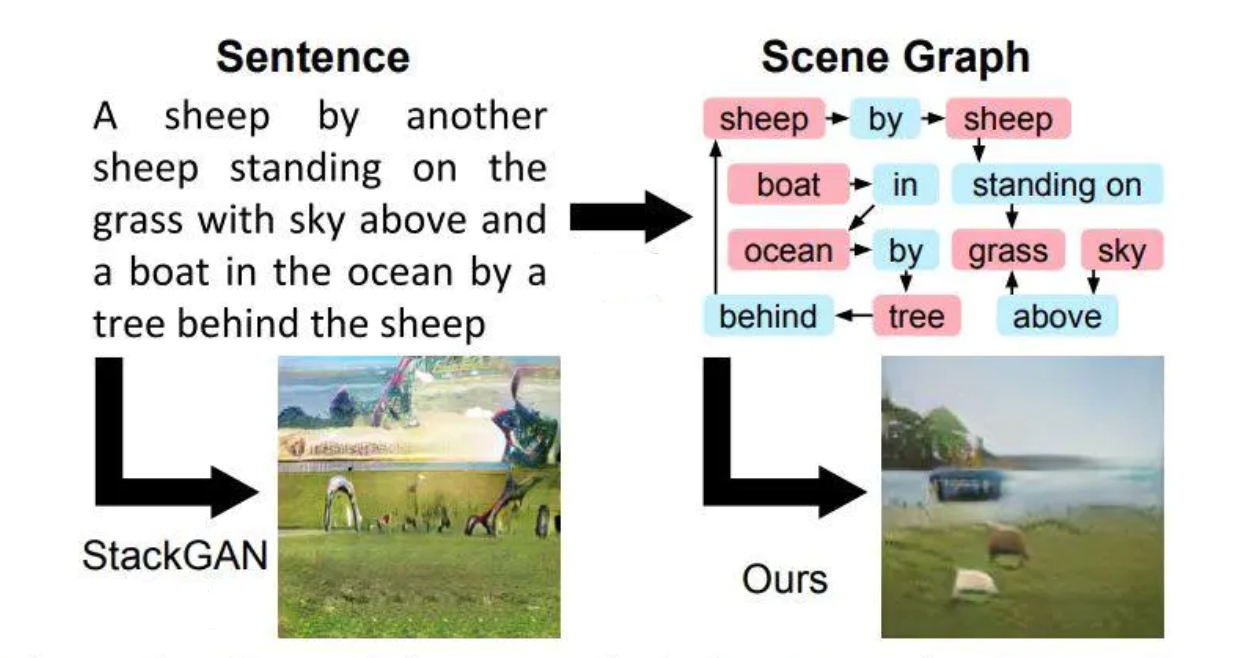
\includegraphics[width=0.8\textwidth]{figures/sg2imcp.png}
    \caption{比较StackGAN和本文算法的生成图像差异}
    \label{fig:sg2imcp}
\end{figure}

有一首小诗\footnote{由文献\cite{Johnson_2018}原作者提出,以解释模型在生成图像方面的优势},因为其包含许多位置关系,非常适合这一算法。以此为例,可以表现此算法对人类主观理解上的优势。

对于如下诗句,StackGAN模型和本文使用模型分别生成了如图~\ref{fig:sg2imcp}的两张截然不同的图像。显然,本文使用模型保留了大部分的位置关系,并且没有产生图像上的扭曲。从人类的视角来看,

A sheep by another sheep

standing on the grass

with sky above and a boat in the ocean

beyond the tree next to the sheep.

另外,在图~\ref{fig:sg2imeg}我们可以清晰地从场景关系图的树状发展流程中,看到构成生成图片的过程。

\begin{figure}[!htbp]
    \centering
    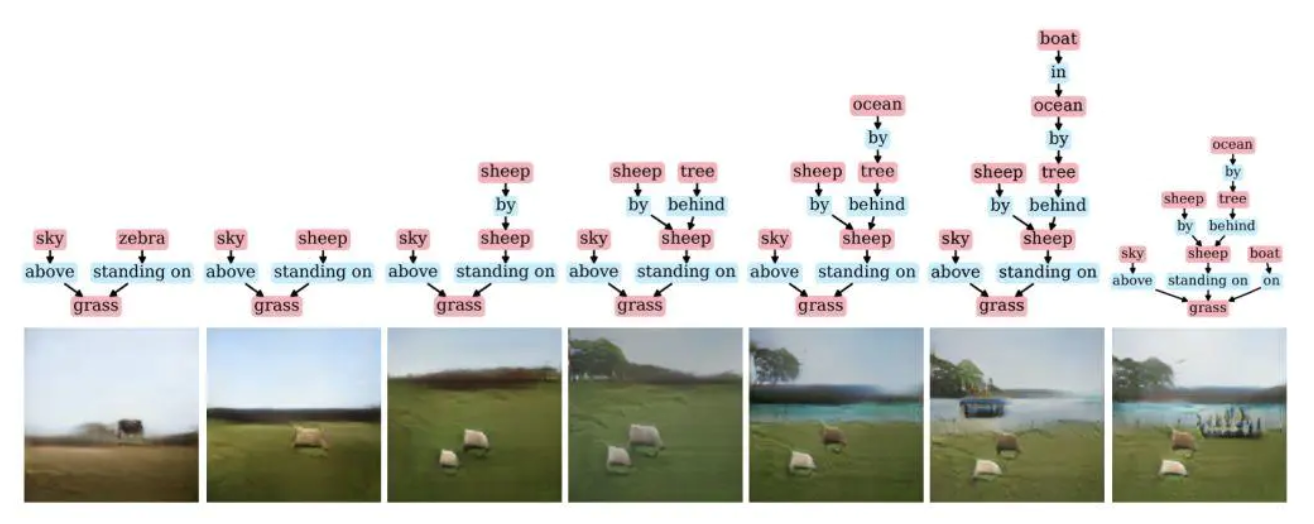
\includegraphics[width=0.8\textwidth]{figures/sg2imeg.png}
    \caption{比较StackGAN和本文算法的生成图像差异}
    \label{fig:sg2imeg}
\end{figure}

\section{本章小结}
这一章节分别介绍了软件界面编码方式、软件两个功能模型训练方式过程与软件部署调试的过程。在软件界面编码中,试用了tkinter进行编码,用比较简明的方式,实现了用例图中的效果;在软件功能模型训练中,记述了LSTM模型和GAN模型分别在环境安装、数据集选取、训练次数调整和呈现方式的过程

%{\songti \bfseries 宋体加粗} {\textbf{English}}

%{\songti \itshape 宋体斜体} {\textit{English}}

%%%{\songti \bfseries \itshape 宋体粗斜体} {\textbf{\textit{English}}}

%\section{编译}
%本模板必须使用XeLaTeX + BibTeX编译,否则会直接报错。 本模板支持多个平台,结合sublime/vscode/overleaf都可以使用。
  % Chapter 5

\chapter{总结与展望}
\section{设计意义}
这一毕业设计题目,是由指导教师通过对课题的理解划分,并结合我所掌握的知识和项目经验,在师生双方通过对题目研究范围、完成任务、达成目标等方面进行探讨后,确定的题目。通过这一设计,既开发了一个有应用价值的软件系统,也活学活用了软件工程、人工智能、机器学习等课程上学习到的知识,为研究生阶段的深造打下了基础。

\subsection{制作了一个简洁易用系统}
设计的成品软件,通过调用模型,可以实现预期的目标:实现自然语言与图像的互译。

图像标注生成文本的部分,使用了2015年Kevin Xu发表的图像字幕方法。这一方法的优势是,它通过编码-解码的方式和注意力机制函数,将图片提取成特征向量,并可以通过长短期记忆模型,生成通顺的简单语句,在实质上完成了图片向自然语言的翻译。

自然语言向图像翻译的部分,使用了李飞飞课题组Johnson在2018年发表在CVPR会议上的基于场景图的图像生成方法。这一方法基于有里程碑意义的StackGAN模型算法,又有了很大的进步。这一算法对生成器提出了很大的优化,使得模型可以在最终的生成图像中,生成很多的物体对象,并且保证它们形状与大小不会产生扭曲、变形,位置关系不会有巨大的谬误。它可以对复杂句说明的场景作出整体的图像生成,这是这个算法的先进性所在。

通过界面制作,将图像测试操作进行了简化,使这一技术应用到了普通人可以随意实用的平台上。

\subsection{活用知识、实践了深度学习技术}
这是我第一次独立一人从环境安装到训练出模型实践一个成熟深度学习算法的复现。

这次的设计使用了本科期间下列几门课程中学到的知识:《软件工程》、《机器学习》、《数据挖掘》等。我在这些课程中学到了深度学习的前置知识与基本概念,为这次成功的实践埋下了伏笔。

在博士研究生阶段,我将在人工智能领域继续探索,这一次的设计为我将来的学习与研究工作打下了扎实的基础。这次成功的实践,不但增强了我的自信,也让我多了一份深度学习项目实践的经验。

\section{未来发展方向}
这一设计还有很大的改进空间。

从界面上说,目前的功能有些单一,样式有些单调。未来可以将注意力信息也输入到界面显示上,为界面增加更多的趣味性与美观。

从图片标注上来说,目前的数据集虽然规模庞大,但是有些单一。经过更多的测试,可以发现对一些色块相似于训练集的图片,容易有过拟合的现象,比如将“road”识别为“river”,或者将建筑物上的花纹识别为“clock”。对于测试集中出现的注意力集中区域识别错误,应当增加相应的数据进行训练。

从文本生成图像上来说,目前的模型在蒙板内的生成物体图像还比较粗糙,另外图片整体的清晰度较低。在$64 \times 64$像素的清晰度下,小物体可能只占几百个或几十个像素点的区域,这样的情况下很难生成让人可以看懂局部的图像,这一点上人类没有判别器做的好,所以保险机制可能不是那么有效。未来可以对每一类别的物体专门训练插值算法模型,加大图像清晰度,让每一个蒙版内的物体图像内容对于自然人的可识别性更好。

%{\songti \bfseries 宋体加粗} {\textbf{English}}

%{\songti \itshape 宋体斜   体} {\textit{English}}

%%%{\songti \bfseries \itshape 宋体粗斜体} {\textbf{\textit{English}}}

%\section{编译}
%本模板必须使用XeLaTeX + BibTeX编译,否则会直接报错。 本模板支持多个平台,结合sublime/vscode/overleaf都可以使用。
  %% Chapter 公式表格样例

\chapter{公式插图表格}

\section{公式的使用}
在文中引用公式可以这么写:$a^2+b^2=c^2$这是勾股定理,他还可以表示为$c=\sqrt{a^2+b^2}$,还可以让公式单独一段并且加上编号。注意,公式前请不要空行。
\begin{equation}
\sin^2{\theta}+\cos^2{\theta}=1 \label{eq:pingfanghe}
\end{equation}

还可以通过添加标签在正文中引用公式,如式\eqref{eq:pingfanghe}。

我们还可以轻松打出一个漂亮的矩阵:
\begin{equation}
  \mathbf{A}=
  \left[\begin{matrix}
    1&2&3&4\\
    11&22&33&44\\
  \end{matrix}\right] \times
  \left[\begin{matrix}
    22&24\\
    32&34\\
    42&44\\
    52&54\\
  \end{matrix}\right]
\end{equation}

或者多行对齐的公式:
\begin{equation}
  \begin{aligned}
    f_1(x)&=(x+y)^2\\
          &=x^2+2xy+y^2
  \end{aligned}
\end{equation}


\section{插图的使用}

\LaTeX 环境下可以使用常见的图片格式:JPEG、PNG、PDF、EPS等。当然也可以使用\LaTeX 直接绘制矢量图形,可以参考pgf/tikz等包中的相关内容。需要注意的是,无论采用什么方式绘制图形,首先考虑的是图片的清晰程度以及图片的可理解性,过于不清晰的图片将可能会浪费很多时间。

图示例如下:

\begin{figure}[!htb]
  \centering
  \includegraphics[width=0.3\textwidth]
  {figures/whulogo.png}\\
  \caption{插图示例}
  \label{fig:whu}
\end{figure}

\verb|[htbp]|选项分别是此处、页顶、页底、独立一页。\verb|[width=\textwidth]|让图片占满整行,或\verb|[width=2cm]|直接设置宽度。可以随时在文中进行引用,如图~\ref{fig:whu},建议缩放时保持图像的宽高比不变。

\section{表格的使用}

表格的输入可能会比较麻烦,可以使用在线的工具,如~\href{https://www.tablesgenerator.com/}{Tables Generator}~能便捷的创建表格,也可以使用离线的工具,如~\href{https://ctan.org/pkg/excel2latex}{Excel2LaTeX}~支持从Excel表格转换成\LaTeX{}表格。\href{https://en.wikibooks.org/wiki/LaTeX/Tables}{LaTeX/Tables}~上及~\href{https://www.tug.org/pracjourn/2007-1/mori/mori.pdf}{Tables in LaTeX}~也有更多的示例能够参考。

\subsection{普通表格}
下面是一些普通表格的示例:

\begin{table}[ht]
  \centering
  \caption{简单表格}
  \label{tab:1}
  \begin{tabular}{|l|c|r|}
    \hline
    我是& 一只 & 普通\\
    \hline
    的& 表格& 呀\\
    \hline
  \end{tabular}
\end{table}

\begin{table}[ht]
  \centering
  \caption{一般三线表}
  \label{tab:2}
  \begin{tabular}{ccc}
    \hline
    姓名& 学号& 性别\\
    \hline
    张三& 001& 男\\
    李四& 002& 女\\
    \hline
  \end{tabular}
\end{table}

\subsection{跨页表格}
跨页表格常用于附录(把正文懒得放下的实验数据统统放在附录的表中),以下是一个跨页表格的示例:

{\centering
  \begin{longtable}{ccccccccc}
  \caption{跨页表格示例} \\
  \toprule
  1     & 0 & 5  & 1  & 2  & 3  & 4  &  5 & 6 \\
  \midrule
  \endfirsthead

  \multicolumn{1}{l}{接上一页} \\
  \toprule
  1     & 0 & 5  & 1  & 2  & 3  & 4  &  5 & 6 \\
  \midrule
  \endhead

  \bottomrule
  \hline \\
  \multicolumn{9}{r}{{转下一页}} \\
  \endfoot

  \bottomrule
  \endlastfoot    

  1     & 0 & 5  & 1  & 2  & 3  & 4  &  5 & 6 \\
  1     & 0 & 5  & 1  & 2  & 3  & 4  &  5 & 6 \\
  1     & 0 & 5  & 1  & 2  & 3  & 4  &  5 & 6 \\
  1     & 0 & 5  & 1  & 2  & 3  & 4  &  5 & 6 \\
  1     & 0 & 5  & 1  & 2  & 3  & 4  &  5 & 6 \\
  1     & 0 & 5  & 1  & 2  & 3  & 4  &  5 & 6 \\
  1     & 0 & 5  & 1  & 2  & 3  & 4  &  5 & 6 \\
  1     & 0 & 5  & 1  & 2  & 3  & 4  &  5 & 6 \\
  1     & 0 & 5  & 1  & 2  & 3  & 4  &  5 & 6 \\
  1     & 0 & 5  & 1  & 2  & 3  & 4  &  5 & 6 \\
  1     & 0 & 5  & 1  & 2  & 3  & 4  &  5 & 6 \\
  1     & 0 & 5  & 1  & 2  & 3  & 4  &  5 & 6 \\

  \end{longtable}
}

\subsection{统计表格}
要创建占满整个文字宽度的表格需要使用到tabularx,如不需要,使用tabular就行。引用表格与其它引用一样,只需要:表~\ref{tab:3},统计表格一般是三线表形式。

\begin{table}[ht]
  \centering
  \caption{统计数据表格}
  \label{tab:3}
  \begin{tabularx}{\textwidth}{CCCC}
    \toprule
    序号&年龄&身高&体重\\
    \midrule
    1&14&156&42\\
    2&16&158&45\\
    3&14&162&48\\
    4&15&163&50\\
    \cmidrule{2-4} %添加2-4列的中线
    平均&15&159.75&46.25\\
    \bottomrule
  \end{tabularx}
\end{table}

\section{列表的使用}
下面演示了创建有序及无序列表,如需其它样式,\href{https://www.latex-tutorial.com/tutorials/lists/}{LaTeX Lists}~上有更多的示例。

\subsection{有序列表}
这是一个计数的列表
  \begin{enumerate}
      \item 第一项
          \begin{enumerate}
              \item 第一项中的第一项
              \item 第一项中的第二项
          \end{enumerate}
      \item 第二项
    \begin{enumerate}[label=(\roman*)]
      \item 第一项中的第一项
      \item 第一项中的第二项
    \end{enumerate}
      \item 第三项
  \end{enumerate}

\subsection{不计数列表}
  这是一个不计数的列表
  \begin{itemize}
      \item 第一项
      \begin{itemize}
          \item 第一项中的第一项
          \item 第一项中的第二项
      \end{itemize}
      \item 第二项
      \item 第三项
  \end{itemize}
  %% 引用

\chapter{其它格式}
\section{代码}
\subsection{原始代码}
朴实的代码块:

使用verbatim可以得到原样的输出,如下:

\begin{verbatim}
    print("Hello world!")
\end{verbatim}

使用\href{https://en.wikibooks.org/wiki/LaTeX/Source_Code_Listings}{listings}环境可以对代码进行进一步的格式化,如下:

\lstset{basicstyle=\ttfamily,breaklines=true}
\begin{lstlisting}[language=Python,frame=single]
import numpy as np

a = np.zeros((2,2))
print(a)
\end{lstlisting}

\subsection{代码高亮}
还可以对代码进行高亮,请参考 \href{https://www.overleaf.com/learn/latex/Code_Highlighting_with_minted}{Code Highlighting with minted}。
请先到cls文件中启用minted库。
注意使用Minted库时,需要系统默认Python有Pygments库,可以通过\verb|$ pip install Pygments| 来进行安装。且需要在编译时加上\verb|--shell-escape|参数,否则会报错。

% \usemintedstyle{vs}
% \begin{minted}[linenos,baselinestretch=1.0,frame=lines]{cpp}
% #include <iostream>
% using namespace std;

% int main() 
% {
%     cout << "Hello, World!";
%     return 0;
% }
% \end{minted}

\subsection{算法描述/伪代码}
参考 \href{https://en.wikibooks.org/wiki/LaTeX/Algorithms}{Algorithms},下面是一个简单的示例:

\begin{algorithm}[H]
  \setstretch{1.5} % 代码间行距设定
  \SetAlgoLined
  \KwResult{Write here the result }
   initialization\;
   \While{While condition}{
    instructions\;
    \eIf{condition}{
     instructions1\;
     }{
     instructions3\;
    }
   }
  \caption{How to write algorithms}
\end{algorithm}

% \begin{algorithm}[]
%   \SetKwInOut{Input}{输入}
%   \SetKwInOut{Output}{输出}
%   \caption{\sc DeepWalk\((G, w, d, \gamma, t)\)}\label{DeepWalk}
%   \Input{图\(G(V,E)\) \\
%     窗大小\(w\) \\
%     嵌入维度\(d\) \\
%     每个节点游走数\(\gamma\) \\
%     游走距离\(t\)
%   }
%   \Output{节点表征矩阵\(\Phi\in\mathbb{R}^{|V|\times d}\)
%   }
%   初始化:从\(\mathcal{U}^{|V|\times d}\)采样\(\Phi\) \\
%   从\(V\)建立二叉树\(T\) \\
%   \For{\(i=0\) to \(\gamma\)}{
%     \(\mathcal{O}\) = Shuffle(\(V\)) \\
%     \ForEach{\(v_i\in\mathcal{O}\)}{
%       \(\mathcal{W}_{v_i}=RandomWalk(G, v_i, t)\) \\
%       \(\textsc{SkipGram}(\Phi, \mathcal{W}_{v_i}, w)\)
%     }
%   }
% \end{algorithm}

\section{绘图}

关于使用 \LaTeX{} 绘图的更多例子,请参考 \href{https://www.overleaf.com/learn/latex/Pgfplots_package}{Pgfplots package} 中的例子。
一般建议使用如Photoshop、PowerPoint等制图,再转换成PDF等格式插入。

\section{写在最后}
工具不重要,对工具的合理运用才重要。希望本模板对大家的论文写作有所帮助。

 
%%----------- 结尾部分 ----------- %%
  \clearpage
  \phantomsection
  \addcontentsline{toc}{chapter}{参考文献}
  \bibliography{ref/refs}   % 参考文献

  % 致谢页

\clearpage
\phantomsection
\addcontentsline{toc}{chapter}{致谢}

\chapter*{致谢}
余撰此文时,春之珞珈或将已矣。月初,余犹叹未有赏樱之缘,月末却复恨
无与折柳之机。

  缘何至此?己亥岁除,荆楚大疫,逾翌年春,染者万计。一时之间,通衢空
继踵之城;四海之内,惶惶闻九州之野。此诚危急存亡之秋也。然,壮士出于兵
破士北,贤明起于大树将颠。乃见国士连夜北上,将扣鲸敌所在;亦闻白衣一苇
渡江,欲治伤痍之重。青丝、白发皆身先士卒,商贾、布衣尽争先解囊。盖闻举
国一心,亦若此也。六旬余,大疫终有治,山河还无恙。此当敬谢天下为先。

而值次大疫,求学之旅即止,每自苦读中惊觉,却恍若隔日。巍巍珞珈,百
年黉门,余求学于此已近四秋矣。惟叹时光不老,韶华难留。余平民世家,聿修
祖德,孝悌累洽,父严母慈。自求学起,徒养余求学之路,予余心存归处,不思
回报,父母之督察,为余顺之成文大有助力。双亲鬓渐发白,然大爱不曾稍减,
于我备至更加。余恨不能为其分忧,不能为其担责,甚为内疚,此余跪而叩谢者
一也。来日,当益勉之学、工作,不负父母谓余之殷殷期!

  恩师李先生晓雷,导余于狭路,示余以通途。本论文之撰写,自题目遴选至
研究思路,自框架结构至细枝末节,皆得先生悉心指点。感荷先生拳拳之心,念
先生之恩重,谢无疆焉!今虽将辞,当不忘师恩,精进图强,以期不失其望也!

  恰同学少年者,皆四海之菁英也。逢风华正茂之时,得遇同窗之谊、金兰之
交、共渡之缘,幸甚至哉!侣缘者谁?

  临书仓卒,谨申数字,用展寸诚,祈恕不恭。书之有尽,敬谢难穷;感慨惶
恐,不知所云。遂以拳拳之心,对吾之恩师、椿萱及列位亲友再致谢忱,    % 致谢
  % 附录

\appendix

\chapter{部分代码}

\section{界面代码}

\section{图片标注主函数代码}

\section{图像生成主函数代码}  % 附录

\end{document}